\chapter{Experiments}

In this chapter we discuss our experiments to evaluate performance of \ac{LVNMT} models with and without normalizing flows. We consider settings to empirically evaluate the impact of latent variables on \ac{LVNMT} systems with attention and language models. We include hyperparameter values in the supplement material Table~\ref{tab:hyperparams}, basing them mostly from \citet{eikema2018AEVNMT}. These hyperparameters were picked primarily with the generative \ac{LVNMT} system in mind, not the discriminative model. However, our main interest is not in the exact gains between models, and empirically these hyperparameters were sufficient. As part of this work, we release our code.\footnote{Experiment code:  https://github.com/gamerDecathlete/NormalizingFlowsNMT}

To help prevent \textit{posterior collapse}, we perform KL-annealing linearly over the first 80,000 mini-batch updates. We choose a word-dropout rate of 0.1 for both models. We note, previous work suggested that word dropout is not necessarily helpful in the discriminative \ac{NMT} case \cite{harshil2018GNMT}. %\reminder{depending on performance of VNMT might move to doing the pretrained trick they describe}

We conducted our experiments with the IWSLT 2016 data sets available in the \textit{torchtext} library.\footnote{https://github.com/pytorch/text} We evaluated our models with the German--English (De--En) language pair. We chose this language direction because we could more naturally evaluate the translations.\footnote{ We did not do any formal human evaluation of translation quality.} This dataset consists of 233,213 training, 2052 validation, and 9773 test sentences. We measure performance with the raw BLEU score implementation available in \textit{sacreBLEU} \cite{post2018SacreBLEU}. For all experiments, we keep the random seed fixed to a single value due to stochastic variables. %, and note that these splits are from the ones available in Torch-Text library. \reminder{move last bit to supplement material, when you do add it also note that with the current TorchText we had to manually combine data as they do not do so with the current implementation}

We represented our vocabulary for each language with \ac{BPE} \cite{sennrich2015NMTRarwordsBPE}. We used vocabularies of 10,000 \ac{BPE}s per language. We found that larger vocabularies resulted in sub-word units that occurred infrequently enough to be uninformative from a practical learning perspective. We performed \ac{BPE} using the \textit{SentencePiece} library.\footnote{https://github.com/google/sentencepiece} We trained our \ac{NMT} models on sequences of maximum length 50. We used beam search with a beam width of 10, and length normalization set to 1.0. Throughout our experiments we will refer to our discriminative models as \ac{VNMT} and our joint system as \ac{GNMT}. % The only other normalizing we did on our data sets was removing diacritics from the Arabic sentences. 


%Although most research in \ac{NMT} literature use beam search decoding, we choose to to use greedy decoding when translating sentences. Our general assumption is that if normalizing flows help with translation, this would carry over to heuristic searchers like beam search. Also, in recent literature studying the impact of beam search, larger beams do not necessarily translate to providing huge improvements in performance \cite{cohen2019unconstrained}. \reminder{ this...is a cop out midly because I saw performance degredation with my beam search algorithm set to 10... it worked fine on a 4,000,000 mil sentence dataset but that took waaaay to long}

%- Our networks use hidden layer sizes and embeddings of size 256 which is similar to the choices made in [eikeman et. al 2018] and we found for VNMT these parameters also worked better than those in [vnmt et. al.] for preliminary experiments on the WMT 2014 data they evaluated on. All specific params are in supplement material.
%We limit ourselves to these datasets, because it allows us to consider multiple language pairs and is a manageable size for our available computation budget. Due to these constraints, we caution readers that our results may not be applicable to datasets of different sizes.

\section{General Translation}

In this section we report our results when including normalizing flows on top of \ac{LVNMT} systems. Our hypothesis was that, given normalizing flows success in computer vision, similar gains can be achieved by including normalizing flows in previously considered \ac{LVNMT} systems.  

%\reminder{ in table 1 dimension of Z = 2, with planar flows set to 2 we get so and so results. (point to cells in table)}
%\reminder{ with latent dim = 2, flows do not really offer any improvement, but if you go with a higher dim space, results suggest adding flows can improve performance. Smaller latent space, GNMT is better without flows, but VNMT benefits from normalizing flows. If we go to higher dimension we start to see some gains with GNMT. Pattern: Planar flows usually do well with a higher number of flows seem to help where as IAF helps with smaller flow }

Our baselines include the \ac{LVNMT} models we described in Chapter 3 with just the diagonal Gaussian for the variational distribution. Our baselines optimize the \ac{ELBO} with an equal number of \ac{MC} samples as our normalizing flows models to provide a fair comparison. This corresponds to better approximations of the negative log-likelihood of sequence predictions. The KL divergence is analytic in the Gaussian case which does not require sampling \cite{kingma2014autoencodingVB,rezende2014stochasticBackprop}. Although we do not report numbers, we did find just increasing the number of \ac{MC} samples improved translation quality on the validation set.

Table \ref{tab:de_en_besttranslations} shows the BLEU score of our results on the test set. The best model was picked based on validation BLEU score from checkpoints after every epoch of training. Each model was trained for 47 epochs.\footnote{An epoch here refers to training on all mini-batches before reshuffling the sentence pairs.} The boldfaced results represent the best performing version of a model for the given latent dimensions and flow type.

Regardless of flow type, we found our generative model to perform better for any number of flows or latent space size. Even our worst performing \ac{GNMT} model (z=128, with 4 Planar flows) provides at least 1.20 BLEU score above the best performing discriminative model (z=128, with 4 \ac{IAF}). This result seems congruent with previous research suggesting joint modelling can be more effective than the simpler discriminative representation \cite{eikema2018AEVNMT}.

We found overall that \ac{VNMT} benefited more from the inclusion of normalizing flows than \ac{GNMT}. For \ac{VNMT}, even a single normalizing flow results in improvements. Between flows, we do not note any clear distinctions for the number of flows or type of flow in the \ac{VNMT} case although best performance included more than just one flow. In contrast, \ac{GNMT} only saw performance gains with a latent space of 256, and even then only a few of the flows models outperformed the baseline. 

Overall these results suggest that flows can indeed be added to existing models and provide benefit to the final translation quality. In several instances our flows models outperform baseline results. Here, it seems the input feeding \ac{VNMT} may benefit more than the initialization approach in our \ac{GNMT} model.

%Our results seem to confirm previous findings on transform complexity, when comparing the flow type for a given number of flows for latent spaces 128 and 256. Generally the \ac{IAF} flows gave higher BLEU score with fewer flows compared to the same number of planar flows. This seems to affirm previous research showing that more complex flows require fewer layers to be beneficial \cite{kingma2016IAF,Berg2018SylvesterNF}. However, as we begin using higher numbers of flows we find that planar flows begin to perform marginally better. This would seem to highlight research suggesting better amortization schemes of flow parameters can generally be beneficial \cite{Berg2018SylvesterNF}, as well the limitations of planar flows transformation capabilities \cite{rezende2015VIwithNF,Berg2018SylvesterNF}.




\begin{table}[] 
	\caption{BLEU score for our models with normalizing flows for German-English (De--En) translation. The best  performances are in bold as compared to differing numbers of flows and the baseline. Yellow rows represent our \ac{VNMT} model results, and red our \ac{GNMT} results for differing number and type of flows. 
		% \reminder{0 flows IS my baseline, explain what your basleines are in. Bold baseline 1 (column explainin it), baseline 2 (column explainin what it is?) }
		 }
	\center
	\label{tab:de_en_besttranslations}
	\begin{tabular}{llllllcl}
		\multicolumn{8}{c}{\textbf{Latent Dimension: 128}}                                                                                                                                                                                                                                                                                                                                                                                                                                                                                                 \\ \hline
		\multicolumn{1}{|l|}{\textbf{Flows}}                          & \multicolumn{1}{l|}{\textbf{1}}                             & \multicolumn{1}{l|}{\textbf{2}}                             & \multicolumn{1}{l|}{\textbf{4}}                             & \multicolumn{1}{l|}{\textbf{8}}                             & \multicolumn{1}{l|}{\textbf{16}}                            & \multicolumn{1}{l|}{\textbf{0 (Baseline)}}                                    & \multicolumn{1}{l|}{\textbf{Model}}                                          \\ \hline
		\rowcolor[HTML]{F9F9E1} 
		\multicolumn{1}{|l|}{\cellcolor[HTML]{F9F9E1}Planar}          & \multicolumn{1}{l|}{\cellcolor[HTML]{F9F9E1}18.84}          & \multicolumn{1}{l|}{\cellcolor[HTML]{F9F9E1}18.84}          & \multicolumn{1}{l|}{\cellcolor[HTML]{F9F9E1}19.14}          & \multicolumn{1}{l|}{\cellcolor[HTML]{F9F9E1}19.02}          & \multicolumn{1}{l|}{\cellcolor[HTML]{F9F9E1}\textbf{19.18}} & \multicolumn{1}{c|}{\cellcolor[HTML]{F9F9E1}}                                 & \multicolumn{1}{l|}{\cellcolor[HTML]{F9F9E1}}                                \\ \cline{1-6}
		\rowcolor[HTML]{F9F9E1} 
		\multicolumn{1}{|l|}{\cellcolor[HTML]{F9F9E1}IAF}             & \multicolumn{1}{l|}{\cellcolor[HTML]{F9F9E1}18.89}          & \multicolumn{1}{l|}{\cellcolor[HTML]{F9F9E1}18.96}          & \multicolumn{1}{l|}{\cellcolor[HTML]{F9F9E1}\textbf{19.29}} & \multicolumn{1}{l|}{\cellcolor[HTML]{F9F9E1}18.81}          & \multicolumn{1}{l|}{\cellcolor[HTML]{F9F9E1}18.92}          & \multicolumn{1}{c|}{\multirow{-2}{*}{\cellcolor[HTML]{F9F9E1}18.768}}         & \multicolumn{1}{l|}{\multirow{-2}{*}{\cellcolor[HTML]{F9F9E1}VNMT}}          \\ \hline
		\rowcolor[HTML]{F4DAD8} 
		\multicolumn{1}{|l|}{\cellcolor[HTML]{F4DAD8}Planar}          & \multicolumn{1}{l|}{\cellcolor[HTML]{F4DAD8}20.59}          & \multicolumn{1}{l|}{\cellcolor[HTML]{F4DAD8}20.60}          & \multicolumn{1}{l|}{\cellcolor[HTML]{F4DAD8}20.48}          & \multicolumn{1}{l|}{\cellcolor[HTML]{F4DAD8}20.55}          & \multicolumn{1}{l|}{\cellcolor[HTML]{F4DAD8}20.66}          & \multicolumn{1}{c|}{\cellcolor[HTML]{F4DAD8}}                                 & \multicolumn{1}{l|}{\cellcolor[HTML]{F4DAD8}}                                \\ \cline{1-6}
		\rowcolor[HTML]{F4DAD8} 
		\multicolumn{1}{|l|}{\cellcolor[HTML]{F4DAD8}IAF}             & \multicolumn{1}{l|}{\cellcolor[HTML]{F4DAD8}20.64}          & \multicolumn{1}{l|}{\cellcolor[HTML]{F4DAD8}20.64}          & \multicolumn{1}{l|}{\cellcolor[HTML]{F4DAD8}20.51}          & \multicolumn{1}{l|}{\cellcolor[HTML]{F4DAD8}20.65}          & \multicolumn{1}{l|}{\cellcolor[HTML]{F4DAD8}20.50}          & \multicolumn{1}{c|}{\multirow{-2}{*}{\cellcolor[HTML]{F4DAD8}\textbf{20.73}}} & \multicolumn{1}{l|}{\multirow{-2}{*}{\cellcolor[HTML]{F4DAD8}GNMT}}          \\ \hline
		\multicolumn{8}{c}{\textbf{Latent Dimension: 256}}                                                                                                                                                                                                                                                                                                                                                                                                                                                                                                 \\ \hline
		\multicolumn{1}{|l|}{\textbf{Flows}}                          & \multicolumn{1}{l|}{\textbf{1}}                             & \multicolumn{1}{l|}{\textbf{2}}                             & \multicolumn{1}{l|}{\textbf{4}}                             & \multicolumn{1}{l|}{\textbf{8}}                             & \multicolumn{1}{l|}{\textbf{16}}                            & \multicolumn{1}{l|}{\textbf{0 (Baseline)}}                                    & \multicolumn{1}{l|}{\textbf{Model}}                                          \\ \hline
		\rowcolor[HTML]{F9F9E1} 
		\multicolumn{1}{|l|}{\cellcolor[HTML]{F9F9E1}Planar} & \multicolumn{1}{l|}{\cellcolor[HTML]{F9F9E1}18.93}          & \multicolumn{1}{l|}{\cellcolor[HTML]{F9F9E1}\textbf{19.26}} & \multicolumn{1}{l|}{\cellcolor[HTML]{F9F9E1}19.02}          & \multicolumn{1}{l|}{\cellcolor[HTML]{F9F9E1}18.80}          & \multicolumn{1}{l|}{\cellcolor[HTML]{F9F9E1}18.82}          & \multicolumn{1}{c|}{\cellcolor[HTML]{F9F9E1}}                                 & \multicolumn{1}{l|}{\cellcolor[HTML]{F9F9E1}}                                \\ \cline{1-6}
		\rowcolor[HTML]{F9F9E1} 
		\multicolumn{1}{|l|}{\cellcolor[HTML]{F9F9E1}IAF}    & \multicolumn{1}{l|}{\cellcolor[HTML]{F9F9E1}18.95}          & \multicolumn{1}{l|}{\cellcolor[HTML]{F9F9E1}\textbf{19.17}} & \multicolumn{1}{l|}{\cellcolor[HTML]{F9F9E1}19.02}          & \multicolumn{1}{l|}{\cellcolor[HTML]{F9F9E1}18.99}          & \multicolumn{1}{l|}{\cellcolor[HTML]{F9F9E1}18.77}          & \multicolumn{1}{c|}{\multirow{-2}{*}{\cellcolor[HTML]{F9F9E1}18.76}}          & \multicolumn{1}{l|}{\multirow{-2}{*}{\cellcolor[HTML]{F9F9E1}VNMT}} \\ \hline
		\rowcolor[HTML]{F4DAD8} 
		\multicolumn{1}{|l|}{\cellcolor[HTML]{F4DAD8}Planar} & \multicolumn{1}{l|}{\cellcolor[HTML]{F4DAD8}20.55}          & \multicolumn{1}{l|}{\cellcolor[HTML]{F4DAD8}\textbf{20.67}} & \multicolumn{1}{l|}{\cellcolor[HTML]{F4DAD8}20.54}          & \multicolumn{1}{l|}{\cellcolor[HTML]{F4DAD8}20.51}          & \multicolumn{1}{l|}{\cellcolor[HTML]{F4DAD8}\textbf{20.67}} & \multicolumn{1}{c|}{\cellcolor[HTML]{F4DAD8}}                                 & \multicolumn{1}{l|}{\cellcolor[HTML]{F4DAD8}}                                \\ \cline{1-6}
		\rowcolor[HTML]{F4DAD8} 
		\multicolumn{1}{|l|}{\cellcolor[HTML]{F4DAD8}IAF}    & \multicolumn{1}{l|}{\cellcolor[HTML]{F4DAD8}20.85}          & \multicolumn{1}{l|}{\cellcolor[HTML]{F4DAD8}\textbf{20.86}} & \multicolumn{1}{l|}{\cellcolor[HTML]{F4DAD8}20.64}          & \multicolumn{1}{l|}{\cellcolor[HTML]{F4DAD8}20.62}          & \multicolumn{1}{l|}{\cellcolor[HTML]{F4DAD8}20.66}          & \multicolumn{1}{c|}{\multirow{-2}{*}{\cellcolor[HTML]{F4DAD8}20.66}}          & \multicolumn{1}{l|}{\multirow{-2}{*}{\cellcolor[HTML]{F4DAD8}GNMT}} \\ \hline
	\end{tabular}
\end{table}

%For our baselines, we train both a VNMT and VAENMT model without normalizing flows. To provide equal comparisons we use the same number of samples as our normalizing flows models. In [Eqn for elbo] this corresponds to better approximations to the negative log-likelihood of sequence predictions as the KL divergence is analytic in the Gaussian case \cite{kingma, }. We consider latent dimensions of 2, 128 [best working latent space in Schulz et. al. 2018 for VNMT], and 256 [value used in Eikman et. al. model]. We consider latent dimensions of 2 as we plot the latent space with normalizing flows, and have previously seen this number of latent dimensions to perform quite well compared to large latent dimensions. We use a linear annealing schedule over the first 2 epochs of training to encourage both models to rely on the latent variables which has been shown to improve overall performance [cite cite cite]. We also try without any annealing to provide a comparison on gains from this annealing. We abstain from using word-dropout which is another regularization technique others have found useful previously to help with some models. Particularly in the VNMT case [GNMT paper] found that it did not help improve performance that particular system. 

%To evaluate our hypothesis, we then include normalizing flows on top of these existing systems keeping everything else in the system fixed. We again consider no annealing and annealing for 2 epochs, and train with N number of samples to approximate the ELBO during the training process. We consider 1, 2, 4, 8, and 16 flows to see if performance improves with an increasing number of flows. We test on the inverse autoregressive flows, and amortized planar flows available in the Pyro library. [might also consider Sylvester flows depending on the results from these...would require a smidge of implementing the amortization].

%We evaluate performance on the BLEU score and also measure the (-ELBO) and NLL during training to determine performance gains from normalizing flows. 




\section{Importance of Attention}

In this section, to investigate the utility of including latent variables, we train simplified versions of our \ac{LVNMT} systems which do not include the attention mechanism. Our motivation for this experiment is to tease apart the impact of our latent variable as the only additional information to the decoding process. We do not expect this system to outperform the models with attention due to their success in \ac{SOTA} models \cite{bahdanau2014NMTBYJoint, vaswani2017attentionTransformer}. However, we hypothesize that if the latent variable can encode useful information in translation, then \ac{NMT} models will still benefit from this global latent information. As an extension, normalizing flows will then enable these variables to be more beneficial by making the latent variable distribution more flexible.

We include the latent variable in the generator network as a substitute for attention, which is the same design choice as \citet{bahdanau2014NMTBYJoint} for including attention. In our previous experiment we did not consider this, as the focus was on incorporating normalizing flows in variations of existing models. We compare our modified discriminative model against a version of \citet{bahdanau2014NMTBYJoint} where attention is simply removed. In the joint modelling case, we compare to a baseline similar to the joint model of \citet{eikema2018AEVNMT} except without attention. Their model optimize the language model and translation systems separately except for sharing the source language word embeddings. All other hyperparameters are the same. In our tables these two modified models are the No Latent (NL) baselines we compare our latent variable models against. Table \ref{tab:de_en_no_attention} show's results for our modified models and the baselines when evaluated with BLEU score. The best performances are bold. They were chosen by comparing models with differing numbers of the same flow, and the baselines.

Considering only the latent dimension size, we find an increase in performance simply doubling the dimensions of the latent variable. This would suggest that bigger latent spaces become more important when the model depends more on the latent variable. The combination of planar flows and \ac{VNMT} seem to benefit most from the latent variable achieving close to our best \ac{GNMT} baseline. Unfortunately, the \ac{IAF} \ac{VNMT} models did not improve as much. There could be several possible reasons. One interpretation we suspect is related to the data conditioning approach of planar flows compared to \ac{IAF}. As our planar flows provide per-sentence flow parameters, this enables them to provide more unique distributions per sentence. In comparison, the \ac{IAF} is unable to capture this more nuanced information by simply conditioning on a context vector. This argument has been pointed out in previous research for other types of flow \cite{Berg2018SylvesterNF}.

Unfortunately, our \ac{GNMT} model did not benefit from the inclusion of normalizing flows and was actually hindered in performance for most choices of flows. We reason this is due to the formulation of \ac{GNMT}. The latent variable initializes the translation system beginning in the encoder network as compared to being passed as input during decoding. Based on our results, it seems this design is less effective compared to the input feeding approach of \ac{VNMT} to utilize latent variables. We conjecture this is likely without explicitly passing $z$ to the decoder, \ac{GNMT} is relying on the \ac{GRU}s to implicitly keep this information from beginning to end. 


\begin{table}[]
	\caption{Results for translation systems without attention mechanism. Baseline includes models with normalizing flows and deterministic version of model excluding latent variables. \ac{VNMT} results are in yellow, and \ac{GNMT} results are in red with best models.  Best models across number and type of flow are in bold. No Latent (NL) are  models trained without z included.
		}
	\label{tab:de_en_no_attention}
	\center
	\begin{tabular}{llllllccl}
		\multicolumn{9}{c}{\textbf{Latent Dimension: 128}}                                                                                                                                                                                                                                                                                                                                                                                                                                                                                                                             \\ \hline
		\multicolumn{1}{|c|}{\textbf{Flows}}                 & \multicolumn{1}{c|}{\textbf{1}}                            & \multicolumn{1}{c|}{\textbf{2}}                   & \multicolumn{1}{c|}{\textbf{4}}                   & \multicolumn{1}{c|}{\textbf{8}}                   & \multicolumn{1}{c|}{\textbf{16}}                           & \multicolumn{1}{c|}{\textbf{0 (Baseline)}}                                   & \multicolumn{1}{c|}{\textbf{NL (Baseline)}}                  & \multicolumn{1}{c|}{\textbf{Model}}                                          \\ \hline
		\rowcolor[HTML]{F9F9E1} 
		\multicolumn{1}{|l|}{\cellcolor[HTML]{F9F9E1}Planar} & \multicolumn{1}{l|}{\cellcolor[HTML]{F9F9E1}6.61}          & \multicolumn{1}{l|}{\cellcolor[HTML]{F9F9E1}6.64} & \multicolumn{1}{l|}{\cellcolor[HTML]{F9F9E1}6.63} & \multicolumn{1}{l|}{\cellcolor[HTML]{F9F9E1}6.93} & \multicolumn{1}{l|}{\cellcolor[HTML]{F9F9E1}\textbf{6.78}} & \multicolumn{1}{c|}{\cellcolor[HTML]{F9F9E1}}                                & \multicolumn{1}{c|}{\cellcolor[HTML]{F9F9E1}}                       & \multicolumn{1}{l|}{\cellcolor[HTML]{F9F9E1}}                                \\ \cline{1-6}
		\rowcolor[HTML]{F9F9E1} 
		\multicolumn{1}{|l|}{\cellcolor[HTML]{F9F9E1}IAF}    & \multicolumn{1}{l|}{\cellcolor[HTML]{F9F9E1}\textbf{6.42}} & \multicolumn{1}{l|}{\cellcolor[HTML]{F9F9E1}6.32} & \multicolumn{1}{l|}{\cellcolor[HTML]{F9F9E1}6.28} & \multicolumn{1}{l|}{\cellcolor[HTML]{F9F9E1}5.98} & \multicolumn{1}{l|}{\cellcolor[HTML]{F9F9E1}5.92}          & \multicolumn{1}{c|}{\multirow{-2}{*}{\cellcolor[HTML]{F9F9E1}6.25}}          & \multicolumn{1}{c|}{\multirow{-2}{*}{\cellcolor[HTML]{F9F9E1}6.38}} & \multicolumn{1}{l|}{\multirow{-2}{*}{\cellcolor[HTML]{F9F9E1}VNMT}}          \\ \hline
		\rowcolor[HTML]{F4DAD8} 
		\multicolumn{1}{|l|}{\cellcolor[HTML]{F4DAD8}Planar} & \multicolumn{1}{l|}{\cellcolor[HTML]{F4DAD8}7.2}           & \multicolumn{1}{l|}{\cellcolor[HTML]{F4DAD8}7.22} & \multicolumn{1}{l|}{\cellcolor[HTML]{F4DAD8}7.19} & \multicolumn{1}{l|}{\cellcolor[HTML]{F4DAD8}7.11} & \multicolumn{1}{l|}{\cellcolor[HTML]{F4DAD8}7.25}          & \multicolumn{1}{c|}{\cellcolor[HTML]{F4DAD8}\textbf{7.37}}                   & \multicolumn{1}{c|}{\cellcolor[HTML]{F4DAD8}}                       & \multicolumn{1}{l|}{\cellcolor[HTML]{F4DAD8}}                                \\ \cline{1-7}
		\rowcolor[HTML]{F4DAD8} 
		\multicolumn{1}{|l|}{\cellcolor[HTML]{F4DAD8}IAF}    & \multicolumn{1}{l|}{\cellcolor[HTML]{F4DAD8}7.31}          & \multicolumn{1}{l|}{\cellcolor[HTML]{F4DAD8}7.37} & \multicolumn{1}{l|}{\cellcolor[HTML]{F4DAD8}7.33} & \multicolumn{1}{l|}{\cellcolor[HTML]{F4DAD8}7.18} & \multicolumn{1}{l|}{\cellcolor[HTML]{F4DAD8}\textbf{7.41}} & \multicolumn{1}{c|}{\cellcolor[HTML]{F4DAD8}7.37}                            & \multicolumn{1}{c|}{\multirow{-2}{*}{\cellcolor[HTML]{F4DAD8}7.16}} & \multicolumn{1}{l|}{\multirow{-2}{*}{\cellcolor[HTML]{F4DAD8}GNMT}}          \\ \hline
		\multicolumn{9}{c}{\textbf{Latent Dimension: 256}}                                                                                                                                                                                                                                                                                                                                                                                                                                                                                                                             \\ \hline
		\multicolumn{1}{|c|}{\textbf{Flows}}                 & \multicolumn{1}{c|}{\textbf{1}}                            & \multicolumn{1}{c|}{\textbf{2}}                   & \multicolumn{1}{c|}{\textbf{4}}                   & \multicolumn{1}{c|}{\textbf{8}}                   & \multicolumn{1}{c|}{\textbf{16}}                           & \multicolumn{1}{c|}{\textbf{0 (Baseline)}}                                   & \multicolumn{1}{c|}{\textbf{NL (Baseline)}}                  & \multicolumn{1}{c|}{\textbf{Model}}                                          \\ \hline
		\rowcolor[HTML]{F9F9E1} 
		\multicolumn{1}{|l|}{\cellcolor[HTML]{F9F9E1}Planar} & \multicolumn{1}{l|}{\cellcolor[HTML]{F9F9E1}6.31}          & \multicolumn{1}{l|}{\cellcolor[HTML]{F9F9E1}6.81} & \multicolumn{1}{l|}{\cellcolor[HTML]{F9F9E1}6.91} & \multicolumn{1}{l|}{\cellcolor[HTML]{F9F9E1}7.37} & \multicolumn{1}{l|}{\cellcolor[HTML]{F9F9E1}\textbf{7.38}} & \multicolumn{1}{c|}{\cellcolor[HTML]{F9F9E1}}                                & \multicolumn{1}{c|}{\cellcolor[HTML]{F9F9E1}}                       & \multicolumn{1}{l|}{\cellcolor[HTML]{F9F9E1}}                                \\ \cline{1-6}
		\rowcolor[HTML]{F9F9E1} 
		\multicolumn{1}{|l|}{\cellcolor[HTML]{F9F9E1}IAF}    & \multicolumn{1}{l|}{\cellcolor[HTML]{F9F9E1}6.45}          & \multicolumn{1}{l|}{\cellcolor[HTML]{F9F9E1}6.47} & \multicolumn{1}{l|}{\cellcolor[HTML]{F9F9E1}6.4}  & \multicolumn{1}{l|}{\cellcolor[HTML]{F9F9E1}6.23} & \multicolumn{1}{l|}{\cellcolor[HTML]{F9F9E1}\textbf{6.71}} & \multicolumn{1}{c|}{\multirow{-2}{*}{\cellcolor[HTML]{F9F9E1}6.43}}          & \multicolumn{1}{c|}{\multirow{-2}{*}{\cellcolor[HTML]{F9F9E1}6.38}} & \multicolumn{1}{l|}{\multirow{-2}{*}{\cellcolor[HTML]{F9F9E1}VNMT}} \\ \hline
		\rowcolor[HTML]{F4DAD8} 
		\multicolumn{1}{|l|}{\cellcolor[HTML]{F4DAD8}Planar} & \multicolumn{1}{l|}{\cellcolor[HTML]{F4DAD8}7.4}           & \multicolumn{1}{l|}{\cellcolor[HTML]{F4DAD8}7.22} & \multicolumn{1}{l|}{\cellcolor[HTML]{F4DAD8}7.33} & \multicolumn{1}{l|}{\cellcolor[HTML]{F4DAD8}7.26} & \multicolumn{1}{l|}{\cellcolor[HTML]{F4DAD8}7.07}          & \multicolumn{1}{c|}{\cellcolor[HTML]{F4DAD8}}                                & \multicolumn{1}{c|}{\cellcolor[HTML]{F4DAD8}}                       & \multicolumn{1}{l|}{\cellcolor[HTML]{F4DAD8}}                                \\ \cline{1-6}
		\rowcolor[HTML]{F4DAD8} 
		\multicolumn{1}{|l|}{\cellcolor[HTML]{F4DAD8}IAF}    & \multicolumn{1}{l|}{\cellcolor[HTML]{F4DAD8}7.35}          & \multicolumn{1}{l|}{\cellcolor[HTML]{F4DAD8}7.34} & \multicolumn{1}{l|}{\cellcolor[HTML]{F4DAD8}7.28} & \multicolumn{1}{l|}{\cellcolor[HTML]{F4DAD8}7.04} & \multicolumn{1}{l|}{\cellcolor[HTML]{F4DAD8}7.36}          & \multicolumn{1}{c|}{\multirow{-2}{*}{\cellcolor[HTML]{F4DAD8}\textbf{7.51}}} & \multicolumn{1}{c|}{\multirow{-2}{*}{\cellcolor[HTML]{F4DAD8}7.16}} & \multicolumn{1}{l|}{\multirow{-2}{*}{\cellcolor[HTML]{F4DAD8}GNMT}} \\ \hline
	\end{tabular}
\end{table}

\section{Understanding Latent Variable} 

%Hypothesis: If the latent variable is encoding information important to the translation process, it stands to reason setting Z = [0, 0 ,.... 0] during the evaluation process will negatively impact translation performance, as otherwise the latent variable z is not encoding useful information in the system.

%Previous research which incorporate latent variables in \ac{NMT} systems have often focused on non-zero KL values as justification for the latent variable encoding information for the generative system. The argument in favor of this metric is that the magnitude of the KL can be used a heuristic to gauge the importance the latent variable plays in the translation system. This stems from the fact that typically the prior is a stationary target and if the KL term is small that the latent variable is uninformative to the system's performance. A limitation of this measurement is that it is not applicable in situation where the prior is learned jointly, such as in our \ac{VNMT} system.

In previous works, the utility of latent variables is typically justified by training a similar system without the latent variable included, or by optimizing the model differently.  In cases where the prior is stationary, authors then typically report the KL divergence to justify the latent variables usage. This metric is inapplicable to \ac{VNMT} where the prior is learned. In the ideal \ac{VNMT} scenario, the KL divergence being 0 suggests both distributions encode the same information.

As an alternative approach to measure the value of our latent variable during translation, we set $z$ to the 0 vector. We measure the difference in BLEU score with and without $z$ during the decoding process. This can give us direct insight into the importance of $z$ when translating sentences, whether the prior is learned or not. Table~\ref{tab:de_en_kl_divergence} provides the KL divergence and Table~\ref{tab:de_en_delta_bleu} shows the difference in BLEU score when z is the 0 vector for our models with attention. 

Interestingly, for many of our \ac{VNMT} models with planar flows we see including $z$ often negatively impacts performance of the translation system. This could suggest that the latent variable itself is not helping the translation, but improves representations in the encoder or source word embeddings. Another explanation is that our substitution of $p_{\theta}$ for $q_{\phi}$ at decode time provide information that is too dissimilar to the variational distribution. This is plausible given that in many cases the KL divergence is non-zero, but even in several instances a lower KL divergence still leads to loss of performance with z (see \ac{VNMT}, z=256 results for 8 flows vs. 16 flows). These substitution approaches have also previously been shown to provide minimal or mixed results in terms of comparative performance \cite{eikema2018AEVNMT}.

The exception to our above observations of course is our \ac{VNMT} with \ac{IAF} models in higher dimensions which seem to heavily depend on the latent variable. One possible reason for this has to do with the amortization of \ac{IAF} flows. As these flows are composed of neural networks shared across data points, they can more easily be viewed as additional layers in the network.\footnote{In a similar setting, one bug we found in our implementation was excluding the projection layer and found similar performance drops to those without \ac{IAF} flows results.} This could also be a more volatile result which occurs due to different choices of initialization. It has been noted KL annealing schemes can be affected by initialization for final performance \cite{sphericallatent2018Xu}.

In comparison, \ac{GNMT} seems to generally show at least minute dependence on the latent variable regardless of number of flows. There do not seem to be any clear patterns between choices about flows and the information encoded by $z$. Likewise, a higher KL divergence does not necessarily correspond to more utility in translation performance.  

When we perform the same experiment with our \ac{LVNMT} systems without attention, we see more dependence on the latent variable for all models. Our results are in Table~\ref{tab:de_en_no_attention_kl_div} and \ref{tab:de_en_no_attention_delta_bleu}. In most cases with planar flows, we see our models depend more on the latent variable over the baseline without planar flows. Our \ac{IAF} flow models are more mixed in terms of performance changes, where in \ac{GNMT} our models depend more on the flows with a smaller latent dimension space as opposed to larger latent space. 

\begin{table}
	\caption{Average KL divergence for the test set. For \ac{VNMT} (yellow) the KL term should be smaller, meaning the distributions encode similar information. For \ac{GNMT} (red) they should be higher as these suggest more informative latent spaces.  }
	\label{tab:de_en_kl_divergence}
	\center
	\begin{tabular}{lccccccl}
		\multicolumn{8}{c}{\textbf{Latent Dimension: 128 (KL Divergence)}}                                                                                                \\ \hline
		\multicolumn{1}{|l|}{\textbf{Flows}}                       & \multicolumn{1}{c|}{\textbf{1}}                   & \multicolumn{1}{c|}{\textbf{2}}                   & \multicolumn{1}{c|}{\textbf{4}}                    & \multicolumn{1}{c|}{\textbf{8}}                   & \multicolumn{1}{c|}{\textbf{16}}                   & \multicolumn{1}{c|}{\textbf{0 (Baseline)}}                          & \multicolumn{1}{l|}{\textbf{Model}}                                          \\ \hline
		\rowcolor[HTML]{F9F9E1} 
		\multicolumn{1}{|l|}{\cellcolor[HTML]{F9F9E1}Planar}       & \multicolumn{1}{c|}{\cellcolor[HTML]{F9F9E1}2.16} & \multicolumn{1}{c|}{\cellcolor[HTML]{F9F9E1}1.27} & \multicolumn{1}{c|}{\cellcolor[HTML]{F9F9E1}1.18}  & \multicolumn{1}{c|}{\cellcolor[HTML]{F9F9E1}1.04} & \multicolumn{1}{c|}{\cellcolor[HTML]{F9F9E1}1.63}  & \multicolumn{1}{c|}{\cellcolor[HTML]{F9F9E1}}                       & \multicolumn{1}{l|}{\cellcolor[HTML]{F9F9E1}}                                \\ \cline{1-6}
		\rowcolor[HTML]{F9F9E1} 
		\multicolumn{1}{|l|}{\cellcolor[HTML]{F9F9E1}IAF}          & \multicolumn{1}{c|}{\cellcolor[HTML]{F9F9E1}0.68} & \multicolumn{1}{c|}{\cellcolor[HTML]{F9F9E1}1.35} & \multicolumn{1}{c|}{\cellcolor[HTML]{F9F9E1}1.32}  & \multicolumn{1}{c|}{\cellcolor[HTML]{F9F9E1}1.6}  & \multicolumn{1}{c|}{\cellcolor[HTML]{F9F9E1}1.06}  & \multicolumn{1}{c|}{\multirow{-2}{*}{\cellcolor[HTML]{F9F9E1}1.04}} & \multicolumn{1}{l|}{\multirow{-2}{*}{\cellcolor[HTML]{F9F9E1}VNMT}}          \\ \hline
		\rowcolor[HTML]{F4DAD8} 
		\multicolumn{1}{|l|}{\cellcolor[HTML]{F4DAD8}Planar}       & \multicolumn{1}{c|}{\cellcolor[HTML]{F4DAD8}3.23} & \multicolumn{1}{c|}{\cellcolor[HTML]{F4DAD8}3.15} & \multicolumn{1}{c|}{\cellcolor[HTML]{F4DAD8}2.36}  & \multicolumn{1}{c|}{\cellcolor[HTML]{F4DAD8}2.82} & \multicolumn{1}{c|}{\cellcolor[HTML]{F4DAD8}3.64}  & \multicolumn{1}{c|}{\cellcolor[HTML]{F4DAD8}}                       & \multicolumn{1}{l|}{\cellcolor[HTML]{F4DAD8}}                                \\ \cline{1-6}
		\rowcolor[HTML]{F4DAD8} 
		\multicolumn{1}{|l|}{\cellcolor[HTML]{F4DAD8}IAF}          & \multicolumn{1}{c|}{\cellcolor[HTML]{F4DAD8}4.31} & \multicolumn{1}{c|}{\cellcolor[HTML]{F4DAD8}4.36} & \multicolumn{1}{c|}{\cellcolor[HTML]{F4DAD8}4.19}  & \multicolumn{1}{c|}{\cellcolor[HTML]{F4DAD8}4.43} & \multicolumn{1}{c|}{\cellcolor[HTML]{F4DAD8}4.14}  & \multicolumn{1}{c|}{\multirow{-2}{*}{\cellcolor[HTML]{F4DAD8}4.39}} & \multicolumn{1}{l|}{\multirow{-2}{*}{\cellcolor[HTML]{F4DAD8}GNMT}}          \\ \hline
		\multicolumn{8}{c}{\textbf{Latent Dimension: 256 (KL Divergence)}}                                                                                                                                                                                                                                                                                                                                                                                                                    \\ \hline
		\multicolumn{1}{|l|}{\textbf{Flows}}                       & \multicolumn{1}{c|}{\textbf{1}}                   & \multicolumn{1}{c|}{\textbf{2}}                   & \multicolumn{1}{c|}{\textbf{4}}                    & \multicolumn{1}{c|}{\textbf{8}}                   & \multicolumn{1}{c|}{\textbf{16}}                   & \multicolumn{1}{c|}{\textbf{0 (Baseline)}}                          & \multicolumn{1}{l|}{\textbf{Model}}                                          \\ \hline
		\rowcolor[HTML]{F9F9E1} 
		\multicolumn{1}{|l|}{\cellcolor[HTML]{F9F9E1}Planar}       & \multicolumn{1}{c|}{\cellcolor[HTML]{F9F9E1}0.92} & \multicolumn{1}{c|}{\cellcolor[HTML]{F9F9E1}2.35} & \multicolumn{1}{c|}{\cellcolor[HTML]{F9F9E1}2.37}  & \multicolumn{1}{c|}{\cellcolor[HTML]{F9F9E1}1.11} & \multicolumn{1}{c|}{\cellcolor[HTML]{F9F9E1}1.27}  & \multicolumn{1}{c|}{\cellcolor[HTML]{F9F9E1}}                       & \multicolumn{1}{c|}{\cellcolor[HTML]{F9F9E1}}                                \\ \cline{1-6}
		\rowcolor[HTML]{F9F9E1} 
		\multicolumn{1}{|l|}{\cellcolor[HTML]{F9F9E1}IAF} & \multicolumn{1}{c|}{\cellcolor[HTML]{F9F9E1}2.41} & \multicolumn{1}{c|}{\cellcolor[HTML]{F9F9E1}1.94} & \multicolumn{1}{c|}{\cellcolor[HTML]{F9F9E1}1.14}  & \multicolumn{1}{c|}{\cellcolor[HTML]{F9F9E1}1.1}  & \multicolumn{1}{c|}{\cellcolor[HTML]{F9F9E1}1.1}   & \multicolumn{1}{c|}{\multirow{-2}{*}{\cellcolor[HTML]{F9F9E1}2.0}}  & \multicolumn{1}{c|}{\multirow{-2}{*}{\cellcolor[HTML]{F9F9E1}VNMT}} \\ \hline
		\rowcolor[HTML]{F4DAD8} 
		\multicolumn{1}{|l|}{\cellcolor[HTML]{F4DAD8}Planar}       & \multicolumn{1}{c|}{\cellcolor[HTML]{F4DAD8}4.34} & \multicolumn{1}{c|}{\cellcolor[HTML]{F4DAD8}3.93} & \multicolumn{1}{c|}{\cellcolor[HTML]{F4DAD8}3.36} & \multicolumn{1}{c|}{\cellcolor[HTML]{F4DAD8}2.75} & \multicolumn{1}{c|}{\cellcolor[HTML]{F4DAD8}3.62} & \multicolumn{1}{c|}{\cellcolor[HTML]{F4DAD8}}                       & \multicolumn{1}{c|}{\cellcolor[HTML]{F4DAD8}}                                \\ \cline{1-6}
		\rowcolor[HTML]{F4DAD8} 
		\multicolumn{1}{|l|}{\cellcolor[HTML]{F4DAD8}IAF} & \multicolumn{1}{c|}{\cellcolor[HTML]{F4DAD8}3.87} & \multicolumn{1}{c|}{\cellcolor[HTML]{F4DAD8}3.74} & \multicolumn{1}{c|}{\cellcolor[HTML]{F4DAD8}4.0}   & \multicolumn{1}{c|}{\cellcolor[HTML]{F4DAD8}3.99} & \multicolumn{1}{c|}{\cellcolor[HTML]{F4DAD8}3.98}  & \multicolumn{1}{c|}{\multirow{-2}{*}{\cellcolor[HTML]{F4DAD8}3.84}} & \multicolumn{1}{c|}{\multirow{-2}{*}{\cellcolor[HTML]{F4DAD8}GNMT}} \\ \hline
	\end{tabular}
\end{table}


\begin{table}[]
	\caption{Change in BLEU score when z is set to 0 vector at decode time. Negative numbers indicate our models do better without z included during translation.}
	\label{tab:de_en_delta_bleu}
	\center
\begin{tabular}{lccccccl}
	\multicolumn{8}{c}{\textbf{Latent Dimension: 128 (BLEU Difference)}}                                                                                                                                                                                                                                                                                                                                                                                                                      \\ \hline
	\multicolumn{1}{|l|}{\textbf{Flows}}                       & \multicolumn{1}{c|}{\textbf{1}}                    & \multicolumn{1}{c|}{\textbf{2}}                    & \multicolumn{1}{c|}{\textbf{4}}                    & \multicolumn{1}{c|}{\textbf{8}}                    & \multicolumn{1}{c|}{\textbf{16}}                   & \multicolumn{1}{c|}{\textbf{0 (Baseline)}}                           & \multicolumn{1}{l|}{\textbf{Model}}                                          \\ \hline
	\rowcolor[HTML]{F9F9E1} 
	\multicolumn{1}{|l|}{\cellcolor[HTML]{F9F9E1}Planar}       & \multicolumn{1}{c|}{\cellcolor[HTML]{F9F9E1}-0.29} & \multicolumn{1}{c|}{\cellcolor[HTML]{F9F9E1}-0.37} & \multicolumn{1}{c|}{\cellcolor[HTML]{F9F9E1}-0.06} & \multicolumn{1}{c|}{\cellcolor[HTML]{F9F9E1}-0.14} & \multicolumn{1}{c|}{\cellcolor[HTML]{F9F9E1}0.1}   & \multicolumn{1}{c|}{\cellcolor[HTML]{F9F9E1}}                        & \multicolumn{1}{l|}{\cellcolor[HTML]{F9F9E1}}                                \\ \cline{1-6}
	\rowcolor[HTML]{F9F9E1} 
	\multicolumn{1}{|l|}{\cellcolor[HTML]{F9F9E1}IAF}          & \multicolumn{1}{c|}{\cellcolor[HTML]{F9F9E1}18.64} & \multicolumn{1}{c|}{\cellcolor[HTML]{F9F9E1}12.17} & \multicolumn{1}{c|}{\cellcolor[HTML]{F9F9E1}15.52} & \multicolumn{1}{c|}{\cellcolor[HTML]{F9F9E1}17.4}  & \multicolumn{1}{c|}{\cellcolor[HTML]{F9F9E1}17.56} & \multicolumn{1}{c|}{\multirow{-2}{*}{\cellcolor[HTML]{F9F9E1}0.04}}  & \multicolumn{1}{l|}{\multirow{-2}{*}{\cellcolor[HTML]{F9F9E1}VNMT}}          \\ \hline
	\rowcolor[HTML]{F4DAD8} 
	\multicolumn{1}{|l|}{\cellcolor[HTML]{F4DAD8}Planar}       & \multicolumn{1}{c|}{\cellcolor[HTML]{F4DAD8}0.14}  & \multicolumn{1}{c|}{\cellcolor[HTML]{F4DAD8}0.08}  & \multicolumn{1}{c|}{\cellcolor[HTML]{F4DAD8}0.02}  & \multicolumn{1}{c|}{\cellcolor[HTML]{F4DAD8}0.06}  & \multicolumn{1}{c|}{\cellcolor[HTML]{F4DAD8}0.1}   & \multicolumn{1}{c|}{\cellcolor[HTML]{F4DAD8}}                        & \multicolumn{1}{l|}{\cellcolor[HTML]{F4DAD8}}                                \\ \cline{1-6}
	\rowcolor[HTML]{F4DAD8} 
	\multicolumn{1}{|l|}{\cellcolor[HTML]{F4DAD8}IAF}          & \multicolumn{1}{c|}{\cellcolor[HTML]{F4DAD8}0.12}  & \multicolumn{1}{c|}{\cellcolor[HTML]{F4DAD8}0.08}  & \multicolumn{1}{c|}{\cellcolor[HTML]{F4DAD8}-0.01} & \multicolumn{1}{c|}{\cellcolor[HTML]{F4DAD8}0.1}   & \multicolumn{1}{c|}{\cellcolor[HTML]{F4DAD8}-0.01} & \multicolumn{1}{c|}{\multirow{-2}{*}{\cellcolor[HTML]{F4DAD8}0.08}}  & \multicolumn{1}{l|}{\multirow{-2}{*}{\cellcolor[HTML]{F4DAD8}GNMT}}          \\ \hline
	\multicolumn{8}{c}{\textbf{Latent Dimension: 256 (BLEU Difference)}}                                                                                                                                                                                                                                                                                                                                                                                                                      \\ \hline
	\multicolumn{1}{|l|}{\textbf{Flows}}                       & \multicolumn{1}{c|}{\textbf{1}}                    & \multicolumn{1}{c|}{\textbf{2}}                    & \multicolumn{1}{c|}{\textbf{4}}                    & \multicolumn{1}{c|}{\textbf{8}}                    & \multicolumn{1}{c|}{\textbf{16}}                   & \multicolumn{1}{c|}{\textbf{0 (Baseline)}}                           & \multicolumn{1}{l|}{\textbf{Model}}                                          \\ \hline
	\rowcolor[HTML]{F9F9E1} 
	\multicolumn{1}{|l|}{\cellcolor[HTML]{F9F9E1}Planar}       & \multicolumn{1}{c|}{\cellcolor[HTML]{F9F9E1}0.02}  & \multicolumn{1}{c|}{\cellcolor[HTML]{F9F9E1}-0.07} & \multicolumn{1}{c|}{\cellcolor[HTML]{F9F9E1}-0.03} & \multicolumn{1}{c|}{\cellcolor[HTML]{F9F9E1}-0.24} & \multicolumn{1}{c|}{\cellcolor[HTML]{F9F9E1}0.16}  & \multicolumn{1}{c|}{\cellcolor[HTML]{F9F9E1}}                        & \multicolumn{1}{c|}{\cellcolor[HTML]{F9F9E1}}                                \\ \cline{1-6}
	\rowcolor[HTML]{F9F9E1} 
	\multicolumn{1}{|l|}{\cellcolor[HTML]{F9F9E1}IAF} & \multicolumn{1}{c|}{\cellcolor[HTML]{F9F9E1}12.22} & \multicolumn{1}{c|}{\cellcolor[HTML]{F9F9E1}17.27} & \multicolumn{1}{c|}{\cellcolor[HTML]{F9F9E1}18.5}  & \multicolumn{1}{c|}{\cellcolor[HTML]{F9F9E1}10.84} & \multicolumn{1}{c|}{\cellcolor[HTML]{F9F9E1}17.42} & \multicolumn{1}{c|}{\multirow{-2}{*}{\cellcolor[HTML]{F9F9E1}-0.11}} & \multicolumn{1}{c|}{\multirow{-2}{*}{\cellcolor[HTML]{F9F9E1}VNMT}} \\ \hline
	\rowcolor[HTML]{F4DAD8} 
	\multicolumn{1}{|l|}{\cellcolor[HTML]{F4DAD8}Planar}       & \multicolumn{1}{c|}{\cellcolor[HTML]{F4DAD8}0.1}   & \multicolumn{1}{c|}{\cellcolor[HTML]{F4DAD8}0}     & \multicolumn{1}{c|}{\cellcolor[HTML]{F4DAD8}0.11}  & \multicolumn{1}{c|}{\cellcolor[HTML]{F4DAD8}0.15}  & \multicolumn{1}{c|}{\cellcolor[HTML]{F4DAD8}0.04}  & \multicolumn{1}{c|}{\cellcolor[HTML]{F4DAD8}}                        & \multicolumn{1}{c|}{\cellcolor[HTML]{F4DAD8}}                                \\ \cline{1-6}
	\rowcolor[HTML]{F4DAD8} 
	\multicolumn{1}{|l|}{\cellcolor[HTML]{F4DAD8}IAF} & \multicolumn{1}{c|}{\cellcolor[HTML]{F4DAD8}0.04}  & \multicolumn{1}{c|}{\cellcolor[HTML]{F4DAD8}0.09}  & \multicolumn{1}{c|}{\cellcolor[HTML]{F4DAD8}0.04}  & \multicolumn{1}{c|}{\cellcolor[HTML]{F4DAD8}0.06}  & \multicolumn{1}{c|}{\cellcolor[HTML]{F4DAD8}0.19}  & \multicolumn{1}{c|}{\multirow{-2}{*}{\cellcolor[HTML]{F4DAD8}0.09}}  & \multicolumn{1}{c|}{\multirow{-2}{*}{\cellcolor[HTML]{F4DAD8}GNMT}} \\ \hline
\end{tabular}
\end{table}



\begin{table}[]
	\caption{Average KL divergence for test set for models without attention. \ac{VNMT} should generally be lower, where as \ac{GNMT} shoulder generally have non-zero KL terms. }
	\label{tab:de_en_no_attention_kl_div}
	\center
\begin{tabular}{llllllccl}
	\multicolumn{9}{c}{\textbf{Latent Dimension: 128 (KL Divergence)}}                                                                                                               \\ \hline
	\multicolumn{1}{|c|}{\textbf{Flows}}                 & \multicolumn{1}{c|}{\textbf{1}}                   & \multicolumn{1}{c|}{\textbf{2}}                   & \multicolumn{1}{c|}{\textbf{4}}                   & \multicolumn{1}{c|}{\textbf{8}}                   & \multicolumn{1}{c|}{\textbf{16}}                  & \multicolumn{1}{c|}{\textbf{0 (Baseline)}}                          & \multicolumn{1}{c|}{\textbf{NL (Baseline)}}                 & \multicolumn{1}{c|}{\textbf{Model}}                                          \\ \hline
	\rowcolor[HTML]{F9F9E1} 
	\multicolumn{1}{|l|}{\cellcolor[HTML]{F9F9E1}Planar} & \multicolumn{1}{l|}{\cellcolor[HTML]{F9F9E1}0.22} & \multicolumn{1}{l|}{\cellcolor[HTML]{F9F9E1}0.56} & \multicolumn{1}{l|}{\cellcolor[HTML]{F9F9E1}0.76} & \multicolumn{1}{l|}{\cellcolor[HTML]{F9F9E1}0.39} & \multicolumn{1}{l|}{\cellcolor[HTML]{F9F9E1}0.05} & \multicolumn{1}{c|}{\cellcolor[HTML]{F9F9E1}}                       & \multicolumn{1}{c|}{\cellcolor[HTML]{F9F9E1}}                      & \multicolumn{1}{l|}{\cellcolor[HTML]{F9F9E1}}                                \\ \cline{1-6}
	\rowcolor[HTML]{F9F9E1} 
	\multicolumn{1}{|l|}{\cellcolor[HTML]{F9F9E1}IAF}    & \multicolumn{1}{l|}{\cellcolor[HTML]{F9F9E1}0.59} & \multicolumn{1}{l|}{\cellcolor[HTML]{F9F9E1}0.39} & \multicolumn{1}{l|}{\cellcolor[HTML]{F9F9E1}0.2}  & \multicolumn{1}{l|}{\cellcolor[HTML]{F9F9E1}0.18} & \multicolumn{1}{l|}{\cellcolor[HTML]{F9F9E1}0.23} & \multicolumn{1}{c|}{\multirow{-2}{*}{\cellcolor[HTML]{F9F9E1}0.6}}  & \multicolumn{1}{c|}{\multirow{-2}{*}{\cellcolor[HTML]{F9F9E1}N/A}} & \multicolumn{1}{l|}{\multirow{-2}{*}{\cellcolor[HTML]{F9F9E1}VNMT}}          \\ \hline
	\rowcolor[HTML]{F4DAD8} 
	\multicolumn{1}{|l|}{\cellcolor[HTML]{F4DAD8}Planar} & \multicolumn{1}{l|}{\cellcolor[HTML]{F4DAD8}4.28} & \multicolumn{1}{l|}{\cellcolor[HTML]{F4DAD8}4.48} & \multicolumn{1}{l|}{\cellcolor[HTML]{F4DAD8}3.84} & \multicolumn{1}{l|}{\cellcolor[HTML]{F4DAD8}4.12} & \multicolumn{1}{l|}{\cellcolor[HTML]{F4DAD8}4.58} & \multicolumn{1}{c|}{\cellcolor[HTML]{F4DAD8}}                       & \multicolumn{1}{c|}{\cellcolor[HTML]{F4DAD8}}                      & \multicolumn{1}{l|}{\cellcolor[HTML]{F4DAD8}}                                \\ \cline{1-6}
	\rowcolor[HTML]{F4DAD8} 
	\multicolumn{1}{|l|}{\cellcolor[HTML]{F4DAD8}IAF}    & \multicolumn{1}{l|}{\cellcolor[HTML]{F4DAD8}3.38} & \multicolumn{1}{l|}{\cellcolor[HTML]{F4DAD8}2.97} & \multicolumn{1}{l|}{\cellcolor[HTML]{F4DAD8}3.89} & \multicolumn{1}{l|}{\cellcolor[HTML]{F4DAD8}4.57} & \multicolumn{1}{l|}{\cellcolor[HTML]{F4DAD8}4.53} & \multicolumn{1}{c|}{\multirow{-2}{*}{\cellcolor[HTML]{F4DAD8}2.23}} & \multicolumn{1}{c|}{\multirow{-2}{*}{\cellcolor[HTML]{F4DAD8}N/A}} & \multicolumn{1}{l|}{\multirow{-2}{*}{\cellcolor[HTML]{F4DAD8}GNMT}}          \\ \hline
	\multicolumn{9}{c}{\textbf{Latent Dimension: 256 (KL Divergence)}}                                                                                                                                                                                                                                                                                                                                                                                                                                                                                 \\ \hline
	\multicolumn{1}{|c|}{\textbf{Flows}}                 & \multicolumn{1}{c|}{\textbf{1}}                   & \multicolumn{1}{c|}{\textbf{2}}                   & \multicolumn{1}{c|}{\textbf{4}}                   & \multicolumn{1}{c|}{\textbf{8}}                   & \multicolumn{1}{c|}{\textbf{16}}                  & \multicolumn{1}{c|}{\textbf{0 (Baseline)}}                          & \multicolumn{1}{c|}{\textbf{NL (Baseline)}}                 & \multicolumn{1}{c|}{\textbf{Model}}                                          \\ \hline
	\rowcolor[HTML]{F9F9E1} 
	\multicolumn{1}{|l|}{\cellcolor[HTML]{F9F9E1}Planar} & \multicolumn{1}{l|}{\cellcolor[HTML]{F9F9E1}0.35} & \multicolumn{1}{l|}{\cellcolor[HTML]{F9F9E1}0.04} & \multicolumn{1}{l|}{\cellcolor[HTML]{F9F9E1}0.3}  & \multicolumn{1}{l|}{\cellcolor[HTML]{F9F9E1}0.16} & \multicolumn{1}{l|}{\cellcolor[HTML]{F9F9E1}0.07} & \multicolumn{1}{c|}{\cellcolor[HTML]{F9F9E1}}                       & \multicolumn{1}{c|}{\cellcolor[HTML]{F9F9E1}}                      & \multicolumn{1}{l|}{\cellcolor[HTML]{F9F9E1}}                                \\ \cline{1-6}
	\rowcolor[HTML]{F9F9E1} 
	\multicolumn{1}{|l|}{\cellcolor[HTML]{F9F9E1}IAF}    & \multicolumn{1}{l|}{\cellcolor[HTML]{F9F9E1}0.74} & \multicolumn{1}{l|}{\cellcolor[HTML]{F9F9E1}0.08} & \multicolumn{1}{l|}{\cellcolor[HTML]{F9F9E1}0.7}  & \multicolumn{1}{l|}{\cellcolor[HTML]{F9F9E1}0.25} & \multicolumn{1}{l|}{\cellcolor[HTML]{F9F9E1}0.22} & \multicolumn{1}{c|}{\multirow{-2}{*}{\cellcolor[HTML]{F9F9E1}0.72}} & \multicolumn{1}{c|}{\multirow{-2}{*}{\cellcolor[HTML]{F9F9E1}N/A}} & \multicolumn{1}{l|}{\multirow{-2}{*}{\cellcolor[HTML]{F9F9E1}VNMT}} \\ \hline
	\rowcolor[HTML]{F4DAD8} 
	\multicolumn{1}{|l|}{\cellcolor[HTML]{F4DAD8}Planar} & \multicolumn{1}{l|}{\cellcolor[HTML]{F4DAD8}4.1}  & \multicolumn{1}{l|}{\cellcolor[HTML]{F4DAD8}4.26} & \multicolumn{1}{l|}{\cellcolor[HTML]{F4DAD8}3.57} & \multicolumn{1}{l|}{\cellcolor[HTML]{F4DAD8}3.54} & \multicolumn{1}{l|}{\cellcolor[HTML]{F4DAD8}3.65} & \multicolumn{1}{c|}{\cellcolor[HTML]{F4DAD8}}                       & \multicolumn{1}{c|}{\cellcolor[HTML]{F4DAD8}}                      & \multicolumn{1}{l|}{\cellcolor[HTML]{F4DAD8}}                                \\ \cline{1-6}
	\rowcolor[HTML]{F4DAD8} 
	\multicolumn{1}{|l|}{\cellcolor[HTML]{F4DAD8}IAF}    & \multicolumn{1}{l|}{\cellcolor[HTML]{F4DAD8}3.99} & \multicolumn{1}{l|}{\cellcolor[HTML]{F4DAD8}3.19} & \multicolumn{1}{l|}{\cellcolor[HTML]{F4DAD8}3.99} & \multicolumn{1}{l|}{\cellcolor[HTML]{F4DAD8}3.12} & \multicolumn{1}{l|}{\cellcolor[HTML]{F4DAD8}3.45} & \multicolumn{1}{c|}{\multirow{-2}{*}{\cellcolor[HTML]{F4DAD8}4.19}} & \multicolumn{1}{c|}{\multirow{-2}{*}{\cellcolor[HTML]{F4DAD8}N/A}} & \multicolumn{1}{l|}{\multirow{-2}{*}{\cellcolor[HTML]{F4DAD8}GNMT}} \\ \hline
\end{tabular}
\end{table}


\begin{table}[]
	\caption{Change in BLEU score without attention models. Positive values indicate latent variable z is important for translation system. All models seem to depend on z when attention is unavailable.}
	\label{tab:de_en_no_attention_delta_bleu}
	\center
\begin{tabular}{llllllccl}
	\multicolumn{9}{c}{\textbf{Latent Dimension: 128 (BLEU Difference)}}                                                                                                                                                                                                                                                                                                                                                                                                                                                                               \\ \hline
	\multicolumn{1}{|c|}{\textbf{Flows}}                 & \multicolumn{1}{c|}{\textbf{1}}                   & \multicolumn{1}{c|}{\textbf{2}}                   & \multicolumn{1}{c|}{\textbf{4}}                   & \multicolumn{1}{c|}{\textbf{8}}                   & \multicolumn{1}{c|}{\textbf{16}}                  & \multicolumn{1}{c|}{\textbf{0 (Baseline)}}                          & \multicolumn{1}{c|}{\textbf{NL (Baseline)}}                 & \multicolumn{1}{c|}{\textbf{Model}}                                          \\ \hline
	\rowcolor[HTML]{F9F9E1} 
	\multicolumn{1}{|l|}{\cellcolor[HTML]{F9F9E1}Planar} & \multicolumn{1}{l|}{\cellcolor[HTML]{F9F9E1}3.02} & \multicolumn{1}{l|}{\cellcolor[HTML]{F9F9E1}3.08} & \multicolumn{1}{l|}{\cellcolor[HTML]{F9F9E1}2.73} & \multicolumn{1}{l|}{\cellcolor[HTML]{F9F9E1}3.51} & \multicolumn{1}{l|}{\cellcolor[HTML]{F9F9E1}3.5}  & \multicolumn{1}{c|}{\cellcolor[HTML]{F9F9E1}}                       & \multicolumn{1}{c|}{\cellcolor[HTML]{F9F9E1}}                      & \multicolumn{1}{l|}{\cellcolor[HTML]{F9F9E1}}                                \\ \cline{1-6}
	\rowcolor[HTML]{F9F9E1} 
	\multicolumn{1}{|l|}{\cellcolor[HTML]{F9F9E1}IAF}    & \multicolumn{1}{l|}{\cellcolor[HTML]{F9F9E1}2.33} & \multicolumn{1}{l|}{\cellcolor[HTML]{F9F9E1}1.75} & \multicolumn{1}{l|}{\cellcolor[HTML]{F9F9E1}1.82} & \multicolumn{1}{l|}{\cellcolor[HTML]{F9F9E1}1.59} & \multicolumn{1}{l|}{\cellcolor[HTML]{F9F9E1}0.88} & \multicolumn{1}{c|}{\multirow{-2}{*}{\cellcolor[HTML]{F9F9E1}0.6}}  & \multicolumn{1}{c|}{\multirow{-2}{*}{\cellcolor[HTML]{F9F9E1}N/A}} & \multicolumn{1}{l|}{\multirow{-2}{*}{\cellcolor[HTML]{F9F9E1}VNMT}}          \\ \hline
	\rowcolor[HTML]{F4DAD8} 
	\multicolumn{1}{|l|}{\cellcolor[HTML]{F4DAD8}Planar} & \multicolumn{1}{l|}{\cellcolor[HTML]{F4DAD8}0.91} & \multicolumn{1}{l|}{\cellcolor[HTML]{F4DAD8}0.93} & \multicolumn{1}{l|}{\cellcolor[HTML]{F4DAD8}0.7}  & \multicolumn{1}{l|}{\cellcolor[HTML]{F4DAD8}0.49} & \multicolumn{1}{l|}{\cellcolor[HTML]{F4DAD8}0.72} & \multicolumn{1}{c|}{\cellcolor[HTML]{F4DAD8}}                       & \multicolumn{1}{c|}{\cellcolor[HTML]{F4DAD8}}                      & \multicolumn{1}{l|}{\cellcolor[HTML]{F4DAD8}}                                \\ \cline{1-6}
	\rowcolor[HTML]{F4DAD8} 
	\multicolumn{1}{|l|}{\cellcolor[HTML]{F4DAD8}IAF}    & \multicolumn{1}{l|}{\cellcolor[HTML]{F4DAD8}0.88} & \multicolumn{1}{l|}{\cellcolor[HTML]{F4DAD8}0.59} & \multicolumn{1}{l|}{\cellcolor[HTML]{F4DAD8}0.88} & \multicolumn{1}{l|}{\cellcolor[HTML]{F4DAD8}0.79} & \multicolumn{1}{l|}{\cellcolor[HTML]{F4DAD8}1.1}  & \multicolumn{1}{c|}{\multirow{-2}{*}{\cellcolor[HTML]{F4DAD8}0.46}} & \multicolumn{1}{c|}{\multirow{-2}{*}{\cellcolor[HTML]{F4DAD8}N/A}} & \multicolumn{1}{l|}{\multirow{-2}{*}{\cellcolor[HTML]{F4DAD8}GNMT}}          \\ \hline
	\multicolumn{9}{c}{\textbf{Latent Dimension: 256 (BLEU Difference)}}                                                                                                                                                                                                                                                                                                                                                                                                                                                                               \\ \hline
	\multicolumn{1}{|c|}{\textbf{Flows}}                 & \multicolumn{1}{c|}{\textbf{1}}                   & \multicolumn{1}{c|}{\textbf{2}}                   & \multicolumn{1}{c|}{\textbf{4}}                   & \multicolumn{1}{c|}{\textbf{8}}                   & \multicolumn{1}{c|}{\textbf{16}}                  & \multicolumn{1}{c|}{\textbf{0 (Baseline)}}                          & \multicolumn{1}{c|}{\textbf{NL (Baseline)}}                 & \multicolumn{1}{c|}{\textbf{Model}}                                          \\ \hline
	\rowcolor[HTML]{F9F9E1} 
	\multicolumn{1}{|l|}{\cellcolor[HTML]{F9F9E1}Planar} & \multicolumn{1}{l|}{\cellcolor[HTML]{F9F9E1}3.15} & \multicolumn{1}{l|}{\cellcolor[HTML]{F9F9E1}4.09} & \multicolumn{1}{l|}{\cellcolor[HTML]{F9F9E1}4.51} & \multicolumn{1}{l|}{\cellcolor[HTML]{F9F9E1}4.88} & \multicolumn{1}{l|}{\cellcolor[HTML]{F9F9E1}4.98} & \multicolumn{1}{c|}{\cellcolor[HTML]{F9F9E1}}                       & \multicolumn{1}{c|}{\cellcolor[HTML]{F9F9E1}}                      & \multicolumn{1}{l|}{\cellcolor[HTML]{F9F9E1}}                                \\ \cline{1-6}
	\rowcolor[HTML]{F9F9E1} 
	\multicolumn{1}{|l|}{\cellcolor[HTML]{F9F9E1}IAF}    & \multicolumn{1}{l|}{\cellcolor[HTML]{F9F9E1}3.03} & \multicolumn{1}{l|}{\cellcolor[HTML]{F9F9E1}3.79} & \multicolumn{1}{l|}{\cellcolor[HTML]{F9F9E1}3.98} & \multicolumn{1}{l|}{\cellcolor[HTML]{F9F9E1}2.29} & \multicolumn{1}{l|}{\cellcolor[HTML]{F9F9E1}3.09} & \multicolumn{1}{c|}{\multirow{-2}{*}{\cellcolor[HTML]{F9F9E1}1.79}} & \multicolumn{1}{c|}{\multirow{-2}{*}{\cellcolor[HTML]{F9F9E1}N/A}} & \multicolumn{1}{l|}{\multirow{-2}{*}{\cellcolor[HTML]{F9F9E1}VNMT}} \\ \hline
	\rowcolor[HTML]{F4DAD8} 
	\multicolumn{1}{|l|}{\cellcolor[HTML]{F4DAD8}Planar} & \multicolumn{1}{l|}{\cellcolor[HTML]{F4DAD8}0.76} & \multicolumn{1}{l|}{\cellcolor[HTML]{F4DAD8}0.98} & \multicolumn{1}{l|}{\cellcolor[HTML]{F4DAD8}0.29} & \multicolumn{1}{l|}{\cellcolor[HTML]{F4DAD8}0.48} & \multicolumn{1}{l|}{\cellcolor[HTML]{F4DAD8}0.51} & \multicolumn{1}{c|}{\cellcolor[HTML]{F4DAD8}}                       & \multicolumn{1}{c|}{\cellcolor[HTML]{F4DAD8}}                      & \multicolumn{1}{l|}{\cellcolor[HTML]{F4DAD8}}                                \\ \cline{1-6}
	\rowcolor[HTML]{F4DAD8} 
	\multicolumn{1}{|l|}{\cellcolor[HTML]{F4DAD8}IAF}    & \multicolumn{1}{l|}{\cellcolor[HTML]{F4DAD8}0.66} & \multicolumn{1}{l|}{\cellcolor[HTML]{F4DAD8}0.5}  & \multicolumn{1}{l|}{\cellcolor[HTML]{F4DAD8}0.63} & \multicolumn{1}{l|}{\cellcolor[HTML]{F4DAD8}0.41} & \multicolumn{1}{l|}{\cellcolor[HTML]{F4DAD8}0.49} & \multicolumn{1}{c|}{\multirow{-2}{*}{\cellcolor[HTML]{F4DAD8}0.68}} & \multicolumn{1}{c|}{\multirow{-2}{*}{\cellcolor[HTML]{F4DAD8}N/A}} & \multicolumn{1}{l|}{\multirow{-2}{*}{\cellcolor[HTML]{F4DAD8}GNMT}} \\ \hline
\end{tabular}
\end{table}

%\begin{figure}
%	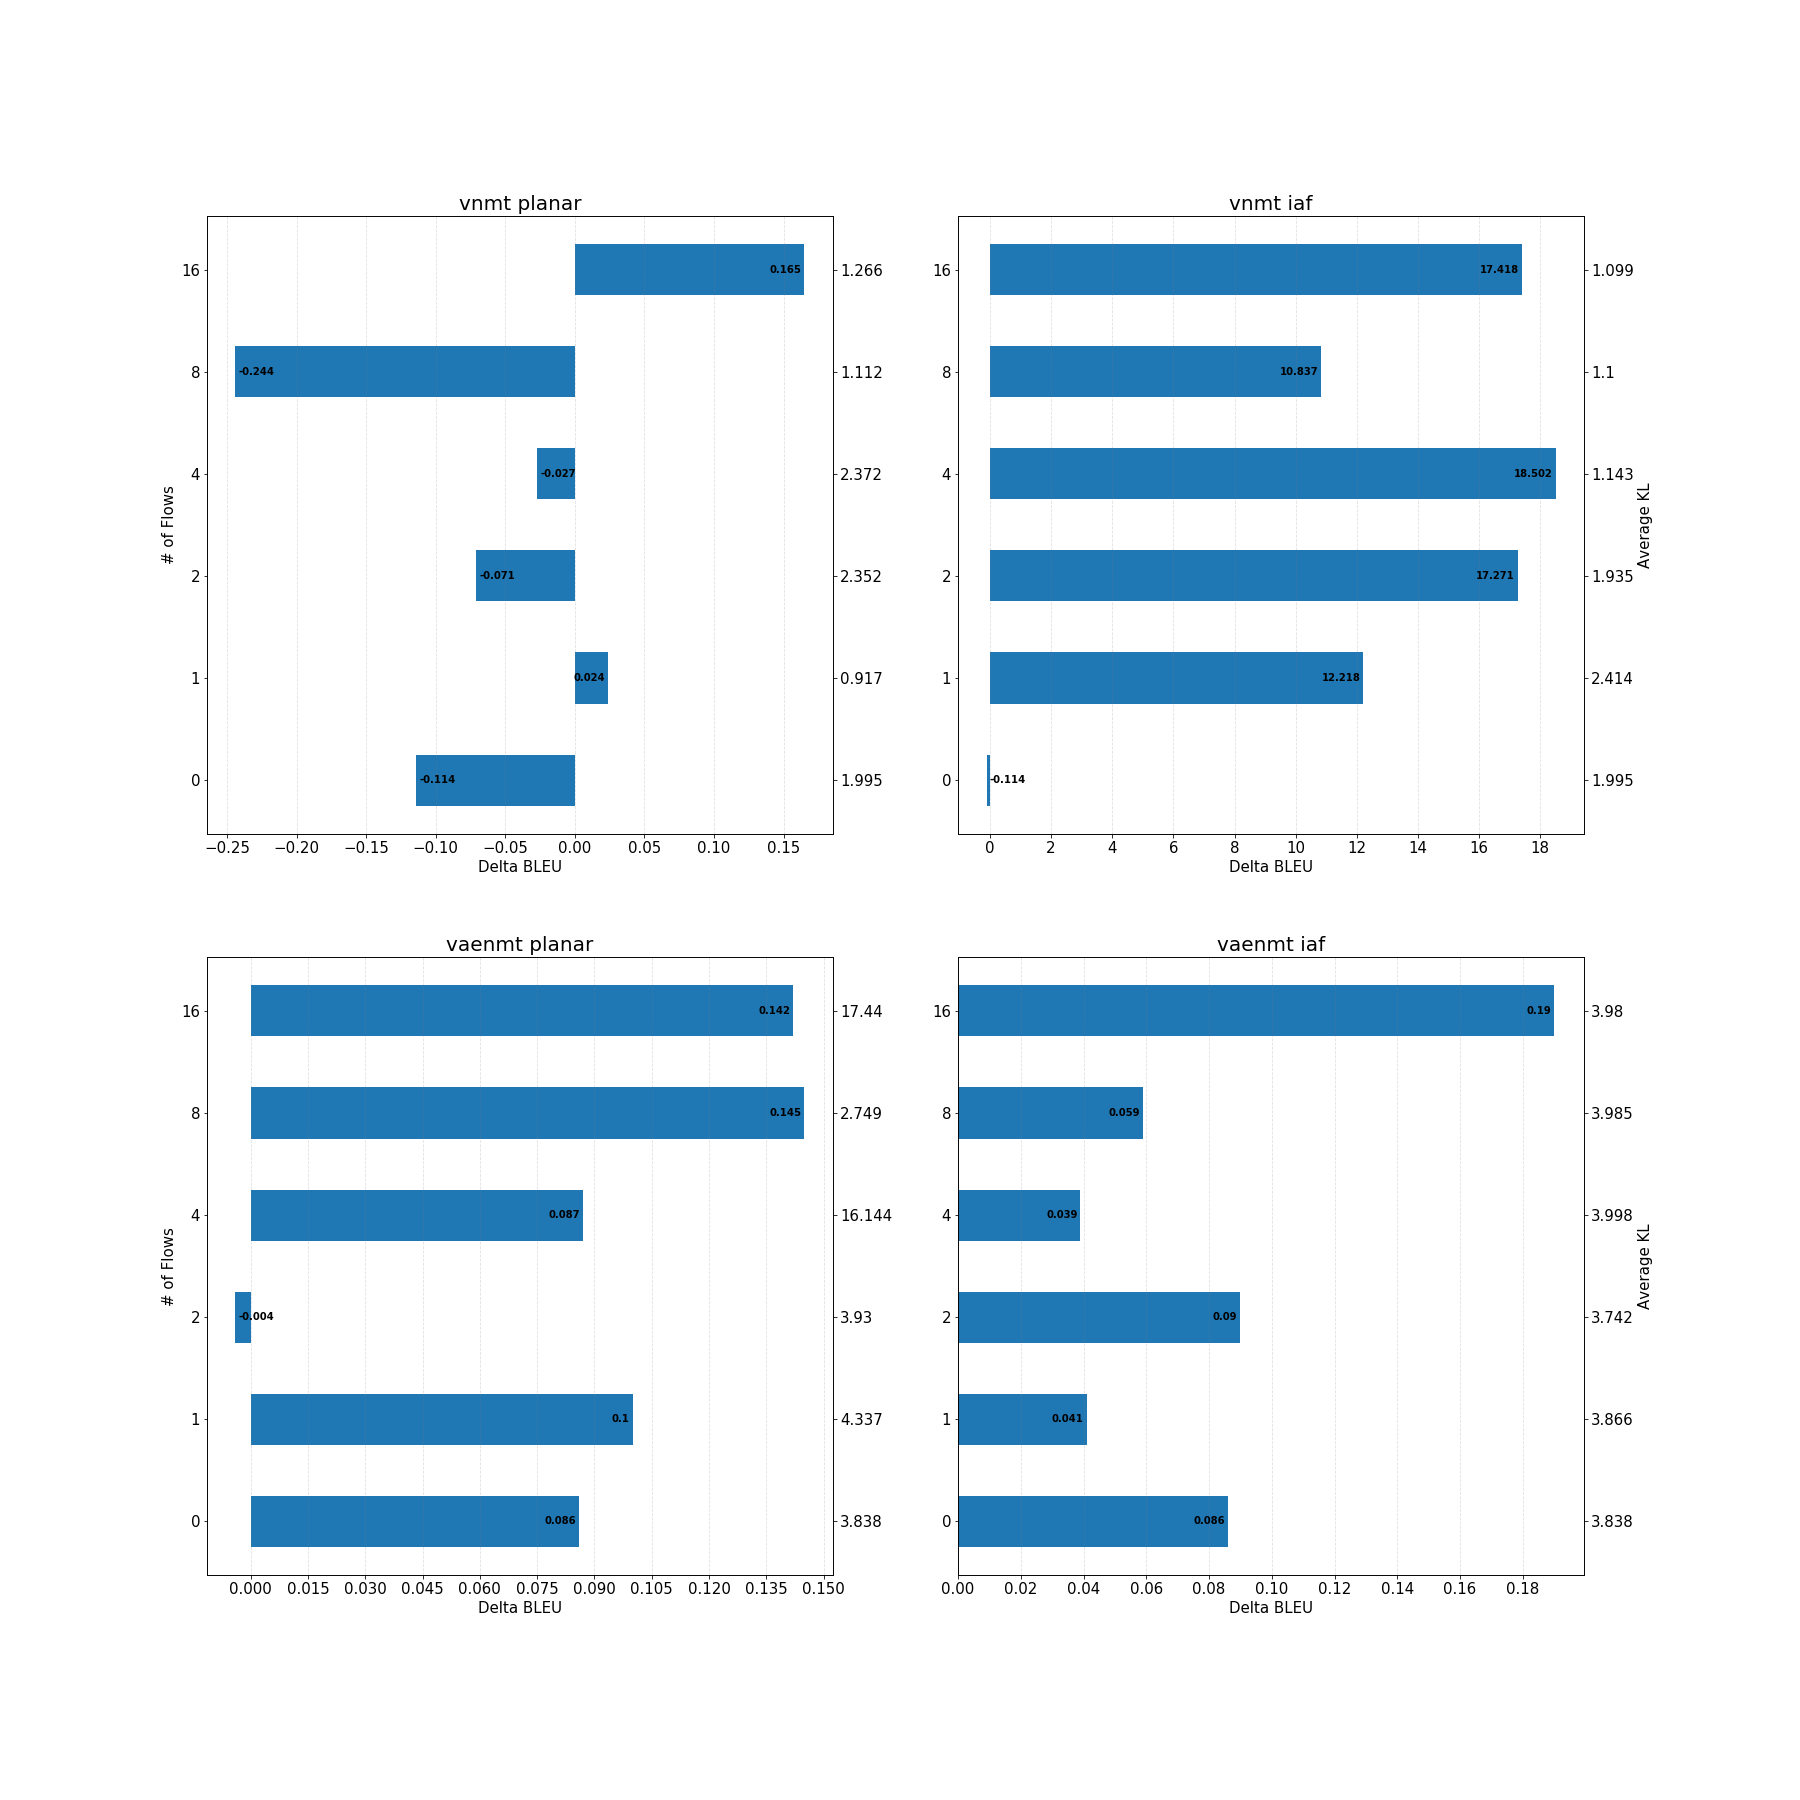
\includegraphics[width=\linewidth]{diff-z-256-horizontalbarplt.png}
%	\caption{The drop in performance when we set the value of the latent variable of Z to 0 during evaluation for latent dimensions set to 256. Bars are $BLEU_{Z=\mu} - BLEU_{Z=0}$. KL divergence of model is included on right axis, number of flows on left axis.}
%	\label{fig:barperfdrop}
%\end{figure}

\section{Language Modelling Performance}

%Hypothesis: Including normalizing flows improve the performance of the language model learned as part of the generative machine translation system. [This is related to a SPECIFIC model and is not applicable to the discriminative version of this stuff...just want to make sure that's clear]
For most of our previous experiments, we have found that \ac{GNMT} largely shows only slight gains from normalizing flows. As previously discussed in chapter 3, \ac{GNMT} trains a language model as part of the system.  In this section, we train \ac{GNMT} models that do not optimize this language model as part of the training procedure. The goal of this experiment is to test the impact of normalizing flows in the absence of language model for \ac{GNMT}.

Table \ref{tab:de_en_vaenmt_bleu_no_lm} shows our results with attention but no language model (in blue) compared against our \ac{GNMT} results from Table~\ref{tab:de_en_besttranslations}. Our results show similar performance to training our \ac{GNMT} model with the language model. At a 128 dimensional latent space our baseline still outperforms all flow models, as well as the training of \ac{GNMT} with a language model. At a 256 latent dimensional space, we see results close to our language model training, but with slight decreases in performance. Given how close these numbers are, these results suggest that $z$ is not the key factor for performance gains in our translation system for \ac{GNMT}. In addition, when we measure the KL divergence (see Table \ref{tab:de_en_vaenmt_bleu_no_lm_kl_divergence} ) we find that the latent variable has largely collapsed to the prior in many cases. Measurements of change of BLEU and without BLEU are in supplementary material Tables~\ref{tab:de_en_kl_divergence_sup}, \ref{tab:de_en_delta_bleu_sup},and  \ref{tab:de_en_vaenmt_bleu_no_lm_delta_bleu_sup}  as these show largely the same behaviour. 

Table \ref{tab:no_attn_no_lm_bleu} shows results of \ac{GNMT} with no language model training along with attention removed.  Here, we see that our flow models show some improvement over baselines unlike the \ac{GNMT} case. The language modelling seems to be more important as \ac{GNMT} does outperform our \ac{GNMT} without language modelling in several cases. Overall though, our best performances in this table is \ac{GNMT} without language modelling and a single planar flow. We did observe \textit{posterior collapse} (included in supplementary material) which might suggest these gains are not directly because of latent variable $z$. This could be simply a by-product of the stochastic behavior due to the training procedure. It has been previously suggested that the stochastic behaviour injected by latent variables does help with training performance \cite{Zhang2016VNMT}. 



\begin{table}[]
	\caption{BLEU scores for \ac{GNMT} without language model training. Bold entries are the best performing models. We include previous \ac{GNMT} results in red to compare with \ac{GNMT} without language model training (blue).}
	\label{tab:de_en_vaenmt_bleu_no_lm}	
	\center
	\begin{tabular}{cccccccc}
		\multicolumn{8}{c}{\textbf{Latent Dimension: 128}}                                                                                                                                                                                                                                                                                                                                                                                                                                                                                                \\ \hline
		\multicolumn{1}{|c|}{\textbf{Flows}}                          & \multicolumn{1}{c|}{\textbf{1}}                             & \multicolumn{1}{c|}{\textbf{2}}                             & \multicolumn{1}{c|}{\textbf{4}}                             & \multicolumn{1}{c|}{\textbf{8}}                    & \multicolumn{1}{c|}{\textbf{16}}                            & \multicolumn{1}{c|}{\textbf{0 (Baseline)}}                                    & \multicolumn{1}{c|}{\textbf{Model}}                                                  \\ \hline
		\rowcolor[HTML]{CEF2F1} 
		\multicolumn{1}{|c|}{\cellcolor[HTML]{CEF2F1}Planar}          & \multicolumn{1}{c|}{\cellcolor[HTML]{CEF2F1}20.46}          & \multicolumn{1}{c|}{\cellcolor[HTML]{CEF2F1}20.42}          & \multicolumn{1}{c|}{\cellcolor[HTML]{CEF2F1}20.5}           & \multicolumn{1}{c|}{\cellcolor[HTML]{CEF2F1}20.65} & \multicolumn{1}{c|}{\cellcolor[HTML]{CEF2F1}20.41}          & \multicolumn{1}{c|}{\cellcolor[HTML]{CEF2F1}}                                 & \multicolumn{1}{c|}{\cellcolor[HTML]{CEF2F1}}                                        \\ \cline{1-6}
		\rowcolor[HTML]{CEF2F1} 
		\multicolumn{1}{|c|}{\cellcolor[HTML]{CEF2F1}IAF}             & \multicolumn{1}{c|}{\cellcolor[HTML]{CEF2F1}20.48}          & \multicolumn{1}{c|}{\cellcolor[HTML]{CEF2F1}20.45}          & \multicolumn{1}{c|}{\cellcolor[HTML]{CEF2F1}20.71}          & \multicolumn{1}{c|}{\cellcolor[HTML]{CEF2F1}20.45} & \multicolumn{1}{c|}{\cellcolor[HTML]{CEF2F1}20.38}          & \multicolumn{1}{c|}{\multirow{-2}{*}{\cellcolor[HTML]{CEF2F1}\textbf{20.77}}} & \multicolumn{1}{c|}{\multirow{-2}{*}{\cellcolor[HTML]{CEF2F1}GNMT (No LM)}}          \\ \hline
		\rowcolor[HTML]{F4DAD8} 
		\multicolumn{1}{|c|}{\cellcolor[HTML]{F4DAD8}Planar}          & \multicolumn{1}{c|}{\cellcolor[HTML]{F4DAD8}20.59}          & \multicolumn{1}{c|}{\cellcolor[HTML]{F4DAD8}20.60}          & \multicolumn{1}{c|}{\cellcolor[HTML]{F4DAD8}20.48}          & \multicolumn{1}{c|}{\cellcolor[HTML]{F4DAD8}20.55} & \multicolumn{1}{c|}{\cellcolor[HTML]{F4DAD8}20.66}          & \multicolumn{1}{c|}{\cellcolor[HTML]{F4DAD8}}                                 & \multicolumn{1}{c|}{\cellcolor[HTML]{F4DAD8}}                                        \\ \cline{1-6}
		\rowcolor[HTML]{F4DAD8} 
		\multicolumn{1}{|c|}{\cellcolor[HTML]{F4DAD8}IAF}             & \multicolumn{1}{c|}{\cellcolor[HTML]{F4DAD8}20.64}          & \multicolumn{1}{c|}{\cellcolor[HTML]{F4DAD8}20.64}          & \multicolumn{1}{c|}{\cellcolor[HTML]{F4DAD8}20.51}          & \multicolumn{1}{c|}{\cellcolor[HTML]{F4DAD8}20.65} & \multicolumn{1}{c|}{\cellcolor[HTML]{F4DAD8}20.50}          & \multicolumn{1}{c|}{\multirow{-2}{*}{\cellcolor[HTML]{F4DAD8}\textbf{20.73}}} & \multicolumn{1}{c|}{\multirow{-2}{*}{\cellcolor[HTML]{F4DAD8}GNMT}}                  \\ \hline
		\multicolumn{8}{c}{\textbf{Latent Dimension: 256}}                                                                                                                                                                                                                                                                                                                                                                                                                                                                                                \\ \hline
		\multicolumn{1}{|c|}{\textbf{Flows}}                          & \multicolumn{1}{c|}{\textbf{1}}                             & \multicolumn{1}{c|}{\textbf{2}}                             & \multicolumn{1}{c|}{\textbf{4}}                             & \multicolumn{1}{c|}{\textbf{8}}                    & \multicolumn{1}{c|}{\textbf{16}}                            & \multicolumn{1}{c|}{\textbf{0 (Baseline)}}                                    & \multicolumn{1}{c|}{\textbf{Model}}                                                  \\ \hline
		\rowcolor[HTML]{CEF2F1} 
		\multicolumn{1}{|c|}{\cellcolor[HTML]{CEF2F1}Planar} & \multicolumn{1}{c|}{\cellcolor[HTML]{CEF2F1}20.32}          & \multicolumn{1}{c|}{\cellcolor[HTML]{CEF2F1}20.36}          & \multicolumn{1}{c|}{\cellcolor[HTML]{CEF2F1}20.47}          & \multicolumn{1}{c|}{\cellcolor[HTML]{CEF2F1}20.21} & \multicolumn{1}{c|}{\cellcolor[HTML]{CEF2F1}\textbf{20.65}} & \multicolumn{1}{c|}{\cellcolor[HTML]{CEF2F1}}                                 & \multicolumn{1}{c|}{\cellcolor[HTML]{CEF2F1}}                                        \\ \cline{1-6}
		\rowcolor[HTML]{CEF2F1} 
		\multicolumn{1}{|c|}{\cellcolor[HTML]{CEF2F1}IAF}    & \multicolumn{1}{c|}{\cellcolor[HTML]{CEF2F1}20.56}          & \multicolumn{1}{c|}{\cellcolor[HTML]{CEF2F1}\textbf{20.64}} & \multicolumn{1}{c|}{\cellcolor[HTML]{CEF2F1}20.51}          & \multicolumn{1}{c|}{\cellcolor[HTML]{CEF2F1}20.54} & \multicolumn{1}{c|}{\cellcolor[HTML]{CEF2F1}20.41}          & \multicolumn{1}{c|}{\multirow{-2}{*}{\cellcolor[HTML]{CEF2F1}20.59}}          & \multicolumn{1}{c|}{\multirow{-2}{*}{\cellcolor[HTML]{CEF2F1}GNMT (No LM)}} \\ \hline
		\rowcolor[HTML]{F4DAD8} 
		\multicolumn{1}{|c|}{\cellcolor[HTML]{F4DAD8}Planar}          & \multicolumn{1}{c|}{\cellcolor[HTML]{F4DAD8}20.55}          & \multicolumn{1}{c|}{\cellcolor[HTML]{F4DAD8}\textbf{20.67}} & \multicolumn{1}{c|}{\cellcolor[HTML]{F4DAD8}20.54}          & \multicolumn{1}{c|}{\cellcolor[HTML]{F4DAD8}20.51} & \multicolumn{1}{c|}{\cellcolor[HTML]{F4DAD8}\textbf{20.67}} & \multicolumn{1}{c|}{\cellcolor[HTML]{F4DAD8}}                                 & \multicolumn{1}{c|}{\cellcolor[HTML]{F4DAD8}}                                        \\ \cline{1-6}
		\rowcolor[HTML]{F4DAD8} 
		\multicolumn{1}{|c|}{\cellcolor[HTML]{F4DAD8}IAF}             & \multicolumn{1}{c|}{\cellcolor[HTML]{F4DAD8}20.85}          & \multicolumn{1}{c|}{\cellcolor[HTML]{F4DAD8}\textbf{20.86}} & \multicolumn{1}{c|}{\cellcolor[HTML]{F4DAD8}20.64}          & \multicolumn{1}{c|}{\cellcolor[HTML]{F4DAD8}20.62} & \multicolumn{1}{c|}{\cellcolor[HTML]{F4DAD8}20.66}          & \multicolumn{1}{c|}{\multirow{-2}{*}{\cellcolor[HTML]{F4DAD8}20.66}}          & \multicolumn{1}{c|}{\multirow{-2}{*}{\cellcolor[HTML]{F4DAD8}GNMT}}                  \\ \hline
	\end{tabular}
\end{table}


\begin{table}[]
	\caption{ \ac{GNMT} training results without attention or language model training. In several instances, \ac{GNMT} without language model training outperform models which optimize the language model. }
	\label{tab:no_attn_no_lm_bleu}
	\center
	\begin{tabular}{cccccccc}
		\multicolumn{8}{c}{\textbf{Latent Dimension: 128}}                                                                                                                                                                                                                                                                                                                                                                                                                                                            \\ \hline
		\multicolumn{1}{|c|}{\textbf{Flows}}                       & \multicolumn{1}{c|}{\textbf{1}}                            & \multicolumn{1}{c|}{\textbf{2}}                   & \multicolumn{1}{c|}{\textbf{4}}                   & \multicolumn{1}{c|}{\textbf{8}}                   & \multicolumn{1}{c|}{\textbf{16}}                           & \multicolumn{1}{c|}{\textbf{0 (Baseline)}}                                   & \multicolumn{1}{c|}{\textbf{Model}}                                         \\ \hline
		\rowcolor[HTML]{CEF2F1} 
		\multicolumn{1}{|c|}{\cellcolor[HTML]{CEF2F1}Planar}       & \multicolumn{1}{c|}{\cellcolor[HTML]{CEF2F1}7.23}          & \multicolumn{1}{c|}{\cellcolor[HTML]{CEF2F1}7.03} & \multicolumn{1}{c|}{\cellcolor[HTML]{CEF2F1}7.25} & \multicolumn{1}{c|}{\cellcolor[HTML]{CEF2F1}\textbf{7.32}} & \multicolumn{1}{c|}{\cellcolor[HTML]{CEF2F1}7.27}          & \multicolumn{1}{c|}{\cellcolor[HTML]{CEF2F1}}                                & \multicolumn{1}{c|}{\cellcolor[HTML]{CEF2F1}}                               \\ \cline{1-6}
		\rowcolor[HTML]{CEF2F1} 
		\multicolumn{1}{|c|}{\cellcolor[HTML]{CEF2F1}IAF}          & \multicolumn{1}{c|}{\cellcolor[HTML]{CEF2F1}\textbf{7.5}}  & \multicolumn{1}{c|}{\cellcolor[HTML]{CEF2F1}7.42} & \multicolumn{1}{c|}{\cellcolor[HTML]{CEF2F1}7.37} & \multicolumn{1}{c|}{\cellcolor[HTML]{CEF2F1}7.31} & \multicolumn{1}{c|}{\cellcolor[HTML]{CEF2F1}7.16}          & \multicolumn{1}{c|}{\multirow{-2}{*}{\cellcolor[HTML]{CEF2F1}7.31}}          & \multicolumn{1}{c|}{\multirow{-2}{*}{\cellcolor[HTML]{CEF2F1}GNMT (No LM)}} \\ \hline
		\rowcolor[HTML]{F4DAD8} 
		\multicolumn{1}{|c|}{\cellcolor[HTML]{F4DAD8}Planar}       & \multicolumn{1}{c|}{\cellcolor[HTML]{F4DAD8}7.2}           & \multicolumn{1}{c|}{\cellcolor[HTML]{F4DAD8}7.22} & \multicolumn{1}{c|}{\cellcolor[HTML]{F4DAD8}7.19} & \multicolumn{1}{c|}{\cellcolor[HTML]{F4DAD8}7.11} & \multicolumn{1}{c|}{\cellcolor[HTML]{F4DAD8}7.25}          & \multicolumn{1}{c|}{\cellcolor[HTML]{F4DAD8}\textbf{7.36}}                   & \multicolumn{1}{c|}{\cellcolor[HTML]{F4DAD8}}                               \\ \cline{1-7}
		\rowcolor[HTML]{F4DAD8} 
		\multicolumn{1}{|c|}{\cellcolor[HTML]{F4DAD8}IAF}          & \multicolumn{1}{c|}{\cellcolor[HTML]{F4DAD8}7.31}          & \multicolumn{1}{c|}{\cellcolor[HTML]{F4DAD8}7.37} & \multicolumn{1}{c|}{\cellcolor[HTML]{F4DAD8}7.33} & \multicolumn{1}{c|}{\cellcolor[HTML]{F4DAD8}7.18} & \multicolumn{1}{c|}{\cellcolor[HTML]{F4DAD8}\textbf{7.41}} & \multicolumn{1}{c|}{\cellcolor[HTML]{F4DAD8}7.36}                            & \multicolumn{1}{c|}{\multirow{-2}{*}{\cellcolor[HTML]{F4DAD8}GNMT}}         \\ \hline
		\multicolumn{8}{c}{\textbf{Latent Dimension: 256}}                                                                                                                                                                                                                                                                                                                                                                                                                                                            \\ \hline
		\multicolumn{1}{|c|}{\textbf{Flows}}                       & \multicolumn{1}{c|}{\textbf{1}}                            & \multicolumn{1}{c|}{\textbf{2}}                   & \multicolumn{1}{c|}{\textbf{4}}                   & \multicolumn{1}{c|}{\textbf{8}}                   & \multicolumn{1}{c|}{\textbf{16}}                           & \multicolumn{1}{c|}{\textbf{0 (Baseline)}}                                   & \multicolumn{1}{c|}{\textbf{Model}}                                         \\ \hline
		\rowcolor[HTML]{CEF2F1} 
		\multicolumn{1}{|c|}{\cellcolor[HTML]{CEF2F1}Planar}       & \multicolumn{1}{c|}{\cellcolor[HTML]{CEF2F1}\textbf{7.58}} & \multicolumn{1}{c|}{\cellcolor[HTML]{CEF2F1}7.45} & \multicolumn{1}{c|}{\cellcolor[HTML]{CEF2F1}7.28} & \multicolumn{1}{c|}{\cellcolor[HTML]{CEF2F1}7.44} & \multicolumn{1}{c|}{\cellcolor[HTML]{CEF2F1}7.33}          & \multicolumn{1}{c|}{\cellcolor[HTML]{CEF2F1}}                                & \multicolumn{1}{c|}{\cellcolor[HTML]{CEF2F1}}                               \\ \cline{1-6}
		\rowcolor[HTML]{CEF2F1} 
		\multicolumn{1}{|c|}{\cellcolor[HTML]{CEF2F1}IAF} & \multicolumn{1}{c|}{\cellcolor[HTML]{CEF2F1}7.25}          & \multicolumn{1}{c|}{\cellcolor[HTML]{CEF2F1}7.35} & \multicolumn{1}{c|}{\cellcolor[HTML]{CEF2F1}7.32} & \multicolumn{1}{c|}{\cellcolor[HTML]{CEF2F1}7.08} & \multicolumn{1}{c|}{\cellcolor[HTML]{CEF2F1}7.47}          & \multicolumn{1}{c|}{\multirow{-2}{*}{\cellcolor[HTML]{CEF2F1}7.21}}          & \multicolumn{1}{c|}{\multirow{-2}{*}{\cellcolor[HTML]{CEF2F1}GNMT (No LM)}} \\ \hline
		\rowcolor[HTML]{F4DAD8} 
		\multicolumn{1}{|c|}{\cellcolor[HTML]{F4DAD8}Planar}       & \multicolumn{1}{c|}{\cellcolor[HTML]{F4DAD8}7.4}           & \multicolumn{1}{c|}{\cellcolor[HTML]{F4DAD8}7.22} & \multicolumn{1}{c|}{\cellcolor[HTML]{F4DAD8}7.33} & \multicolumn{1}{c|}{\cellcolor[HTML]{F4DAD8}7.26} & \multicolumn{1}{c|}{\cellcolor[HTML]{F4DAD8}7.07}          & \multicolumn{1}{c|}{\cellcolor[HTML]{F4DAD8}}                                & \multicolumn{1}{c|}{\cellcolor[HTML]{F4DAD8}}                               \\ \cline{1-6}
		\rowcolor[HTML]{F4DAD8} 
		\multicolumn{1}{|c|}{\cellcolor[HTML]{F4DAD8}IAF}          & \multicolumn{1}{c|}{\cellcolor[HTML]{F4DAD8}7.35}          & \multicolumn{1}{c|}{\cellcolor[HTML]{F4DAD8}7.34} & \multicolumn{1}{c|}{\cellcolor[HTML]{F4DAD8}7.28} & \multicolumn{1}{c|}{\cellcolor[HTML]{F4DAD8}7.04} & \multicolumn{1}{c|}{\cellcolor[HTML]{F4DAD8}7.36}          & \multicolumn{1}{c|}{\multirow{-2}{*}{\cellcolor[HTML]{F4DAD8}\textbf{7.51}}} & \multicolumn{1}{c|}{\multirow{-2}{*}{\cellcolor[HTML]{F4DAD8}GNMT}}         \\ \hline
	\end{tabular}
\end{table}





\begin{table}[]
	\caption{KL divergence of \ac{GNMT} models without language model training. Typically a near 0 KL divergence with stationary priors indicates \textit{posterior collapse} has occurred.  }
	\label{tab:de_en_vaenmt_bleu_no_lm_kl_divergence}
	\center	
	\begin{tabular}{cccccccc}
		\multicolumn{8}{c}{\textbf{Latent Dimension: 128 (KL Divergence)}}                                                                                                                                                                                                                                                                                                                                                                                                                             \\ \hline
		\multicolumn{1}{|c|}{\textbf{Flows}}                          & \multicolumn{1}{c|}{\textbf{1}}                   & \multicolumn{1}{c|}{\textbf{2}}                   & \multicolumn{1}{c|}{\textbf{4}}                   & \multicolumn{1}{c|}{\textbf{8}}                   & \multicolumn{1}{c|}{\textbf{16}}                  & \multicolumn{1}{c|}{\textbf{0 (Baseline)}}                          & \multicolumn{1}{c|}{\textbf{Model}}                                                  \\ \hline
		\rowcolor[HTML]{CEF2F1} 
		\multicolumn{1}{|c|}{\cellcolor[HTML]{CEF2F1}Planar}          & \multicolumn{1}{c|}{\cellcolor[HTML]{CEF2F1}0.01} & \multicolumn{1}{c|}{\cellcolor[HTML]{CEF2F1}0.0}  & \multicolumn{1}{c|}{\cellcolor[HTML]{CEF2F1}0.0}  & \multicolumn{1}{c|}{\cellcolor[HTML]{CEF2F1}0.01} & \multicolumn{1}{c|}{\cellcolor[HTML]{CEF2F1}0.01} & \multicolumn{1}{c|}{\cellcolor[HTML]{CEF2F1}}                       & \multicolumn{1}{c|}{\cellcolor[HTML]{CEF2F1}}                                        \\ \cline{1-6}
		\rowcolor[HTML]{CEF2F1} 
		\multicolumn{1}{|c|}{\cellcolor[HTML]{CEF2F1}IAF}             & \multicolumn{1}{c|}{\cellcolor[HTML]{CEF2F1}0.0}  & \multicolumn{1}{c|}{\cellcolor[HTML]{CEF2F1}0.0}  & \multicolumn{1}{c|}{\cellcolor[HTML]{CEF2F1}0.0}  & \multicolumn{1}{c|}{\cellcolor[HTML]{CEF2F1}0.01} & \multicolumn{1}{c|}{\cellcolor[HTML]{CEF2F1}0.01} & \multicolumn{1}{c|}{\multirow{-2}{*}{\cellcolor[HTML]{CEF2F1}0.0}}  & \multicolumn{1}{c|}{\multirow{-2}{*}{\cellcolor[HTML]{CEF2F1}GNMT (No LM)}}          \\ \hline
		\rowcolor[HTML]{F4DAD8} 
		\multicolumn{1}{|c|}{\cellcolor[HTML]{F4DAD8}Planar}          & \multicolumn{1}{c|}{\cellcolor[HTML]{F4DAD8}3.23} & \multicolumn{1}{c|}{\cellcolor[HTML]{F4DAD8}3.15} & \multicolumn{1}{c|}{\cellcolor[HTML]{F4DAD8}2.36} & \multicolumn{1}{c|}{\cellcolor[HTML]{F4DAD8}2.82} & \multicolumn{1}{c|}{\cellcolor[HTML]{F4DAD8}3.64} & \multicolumn{1}{c|}{\cellcolor[HTML]{F4DAD8}}                       & \multicolumn{1}{c|}{\cellcolor[HTML]{F4DAD8}}                                        \\ \cline{1-6}
		\rowcolor[HTML]{F4DAD8} 
		\multicolumn{1}{|c|}{\cellcolor[HTML]{F4DAD8}IAF}             & \multicolumn{1}{c|}{\cellcolor[HTML]{F4DAD8}4.31} & \multicolumn{1}{c|}{\cellcolor[HTML]{F4DAD8}4.36} & \multicolumn{1}{c|}{\cellcolor[HTML]{F4DAD8}4.19} & \multicolumn{1}{c|}{\cellcolor[HTML]{F4DAD8}4.43} & \multicolumn{1}{c|}{\cellcolor[HTML]{F4DAD8}4.14} & \multicolumn{1}{c|}{\multirow{-2}{*}{\cellcolor[HTML]{F4DAD8}4.39}} & \multicolumn{1}{c|}{\multirow{-2}{*}{\cellcolor[HTML]{F4DAD8}GNMT}}                  \\ \hline
		\multicolumn{8}{c}{\textbf{Latent Dimension: 256  (KL Divergence)}}                                                                                                                                                                                                                                                                                                                                                                                                                            \\ \hline
		\multicolumn{1}{|c|}{\textbf{Flows}}                          & \multicolumn{1}{c|}{\textbf{1}}                   & \multicolumn{1}{c|}{\textbf{2}}                   & \multicolumn{1}{c|}{\textbf{4}}                   & \multicolumn{1}{c|}{\textbf{8}}                   & \multicolumn{1}{c|}{\textbf{16}}                  & \multicolumn{1}{c|}{\textbf{0 (Baseline)}}                          & \multicolumn{1}{c|}{\textbf{Model}}                                                  \\ \hline
		\rowcolor[HTML]{CEF2F1} 
		\multicolumn{1}{|c|}{\cellcolor[HTML]{CEF2F1}Planar} & \multicolumn{1}{c|}{\cellcolor[HTML]{CEF2F1}0.01} & \multicolumn{1}{c|}{\cellcolor[HTML]{CEF2F1}0.01} & \multicolumn{1}{c|}{\cellcolor[HTML]{CEF2F1}0.01} & \multicolumn{1}{c|}{\cellcolor[HTML]{CEF2F1}0.01} & \multicolumn{1}{c|}{\cellcolor[HTML]{CEF2F1}0.01} & \multicolumn{1}{c|}{\cellcolor[HTML]{CEF2F1}}                       & \multicolumn{1}{c|}{\cellcolor[HTML]{CEF2F1}}                                        \\ \cline{1-6}
		\rowcolor[HTML]{CEF2F1} 
		\multicolumn{1}{|c|}{\cellcolor[HTML]{CEF2F1}IAF}    & \multicolumn{1}{c|}{\cellcolor[HTML]{CEF2F1}0.0}  & \multicolumn{1}{c|}{\cellcolor[HTML]{CEF2F1}0.0}  & \multicolumn{1}{c|}{\cellcolor[HTML]{CEF2F1}0.0}  & \multicolumn{1}{c|}{\cellcolor[HTML]{CEF2F1}0.0}  & \multicolumn{1}{c|}{\cellcolor[HTML]{CEF2F1}0.01} & \multicolumn{1}{c|}{\multirow{-2}{*}{\cellcolor[HTML]{CEF2F1}0.0}}  & \multicolumn{1}{c|}{\multirow{-2}{*}{\cellcolor[HTML]{CEF2F1}GNMT (No LM)}} \\ \hline
		\rowcolor[HTML]{F4DAD8} 
		\multicolumn{1}{|c|}{\cellcolor[HTML]{F4DAD8}Planar}          & \multicolumn{1}{c|}{\cellcolor[HTML]{F4DAD8}4.34} & \multicolumn{1}{c|}{\cellcolor[HTML]{F4DAD8}3.93} & \multicolumn{1}{c|}{\cellcolor[HTML]{F4DAD8}3.36} & \multicolumn{1}{c|}{\cellcolor[HTML]{F4DAD8}2.75} & \multicolumn{1}{c|}{\cellcolor[HTML]{F4DAD8}3.62} & \multicolumn{1}{c|}{\cellcolor[HTML]{F4DAD8}}                       & \multicolumn{1}{c|}{\cellcolor[HTML]{F4DAD8}}                                        \\ \cline{1-6}
		\rowcolor[HTML]{F4DAD8} 
		\multicolumn{1}{|c|}{\cellcolor[HTML]{F4DAD8}IAF}             & \multicolumn{1}{c|}{\cellcolor[HTML]{F4DAD8}3.87} & \multicolumn{1}{c|}{\cellcolor[HTML]{F4DAD8}3.74} & \multicolumn{1}{c|}{\cellcolor[HTML]{F4DAD8}4.0}  & \multicolumn{1}{c|}{\cellcolor[HTML]{F4DAD8}3.99} & \multicolumn{1}{c|}{\cellcolor[HTML]{F4DAD8}3.98} & \multicolumn{1}{c|}{\multirow{-2}{*}{\cellcolor[HTML]{F4DAD8}3.84}} & \multicolumn{1}{c|}{\multirow{-2}{*}{\cellcolor[HTML]{F4DAD8}GNMT}}                  \\ \hline
	\end{tabular}
\end{table}




